%\documentclass[draft]{ua-thesis}
\documentclass[final]{ua-thesis}
\usepackage{multirow}
\usepackage[section] {placeins}
\usepackage{setspace}
%\onehalfspacing
%\doublespacing

% this package allows insertion of entire pdfs
\usepackage[final]{pdfpages}

%\linespread{1.75}
%\addtolength{\footskip}{24 pt}  % pushes page no. down at bottom of page

%\usepackage[breaklinks]{hyperref}
\usepackage{graphicx}
\usepackage{amsmath,amsfonts,amssymb}
\usepackage{amsthm}
%\usepackage{soul}  %for underline characters
\usepackage{natbib}
\bibliographystyle{newapa}
%\bibliographystyle{unsrtnat}
\bibpunct{(}{)}{;}{a}{,}{,}
%\usepackage[backend=biber,style=authoryear,citestyle=authoryear,sorting=none]{biblatex}
%\usepackage[backend=biber,style=apa,citestyle=apa,sorting=none]{biblatex}
%\bibliography{/Users/grantschissler/Dropbox/bib/default,/Users/grantschissler/Dropbox/bib/library}
%\defbibheading{refs}[refs]{%
%\chapter*{References}%
%}
%\DeclareSourcemap{
%  \maps[datatype=bibtex, overwrite]{
%    \map{
%      \step[fieldset=url, null]
%    }
%  }
%}
%

\newtheorem{definition}{Definition}[section] %For definition and numbered in sections
\numberwithin{equation}{section}
%\numberwithin{table}{subsection}
%\numberwithin{figure}{subsection}

%\long\def\symbolfootnote[#1]#2{\begingroup% For special symbols in footnote
%\def\thefootnote{\fnsymbol{footnote}}\footnote[#1]{#2}\endgroup}

%\setlength{\topmargin}{0in}
%\setlength{\textheight}{8.5in}
%\setlength{\evensidemargin}{0in}
%\setlength{\oddsidemargin}{0in}
%\setlength{\textwidth}{6.5in}

\newcommand\solidrule[1][1cm]{\rule[0.5ex]{#1}{.4pt}}
\newcommand\dottedrule{\mbox{%
\solidrule[.3mm]\hspace{.7mm}\solidrule[.3mm]\hspace{.7mm}\solidrule[.3mm]\hspace{.7mm}\solidrule[.3mm]\hspace{.7mm}\solidrule[.3mm]\hspace{.7mm}%
\solidrule[.3mm]\hspace{.7mm}\solidrule[.3mm]\hspace{.7mm}\solidrule[.3mm]\hspace{.7mm}\solidrule[.3mm]\hspace{.7mm}\solidrule[.3mm]\hspace{.7mm}}}
\newcommand\dashedrule{\mbox{%
\solidrule[1mm]\hspace{1mm}\solidrule[1mm]\hspace{1mm}\solidrule[1mm]\hspace{1mm}\solidrule[1mm]\hspace{1mm}\solidrule[1mm]\hspace{1mm}}}
\newcommand\dasheddotted{\mbox{%
\solidrule[1mm]\hspace{.4mm}\solidrule[.2mm]\hspace{.4mm}\solidrule[1mm]\hspace{.4mm}\solidrule[.2mm]\hspace{.4mm}%
\solidrule[1mm]\hspace{.4mm}\solidrule[.2mm]\hspace{.4mm}\solidrule[1mm]\hspace{.4mm}\solidrule[.2mm]\hspace{.4mm}%
\solidrule[1mm]\hspace{.4mm}\solidrule[.2mm]\hspace{.4mm}}}

\director{Walter W.~Piegorsch \& Yves A.~Lussier}
\author{Alfred Grant Schissler}
% \title{Statistical and Bioinformatic Contributions to Single-Subject Transcriptome Analytics}
\title{contributions to gene set analysis of correlated, paired-sample transcriptome data to enable precision medicine}
\date{2017}
    \makeindex

%\ifpdf \pdfinfo{ /Author (Qijun Fang) /Title  (Hierarchical Bayesian Benchmark Dose Analysis) } \fi


\begin{document}
\maketitle

\chapter*{Acknowledgments}
First and foremost, I would like to express my heartfelt gratitude towards my co-advisors, Dr. Walter W Piegorsch and Dr. Yves A Lussier. Both have invested countless hours in my training and provided me with unique tools, experience, and perspectives. From Yves, I learned what it takes to produce rapidly in an academic environment. His knowledge, determination, creativity, and commitment to biomedical science is inspiring. From Walt, I am finally beginning to ``think like a statistician'', a gift which was my motivation for this graduate experience. His ability to explain statistical ideas through his writing and presentation is truly amazing. His creativity, curiosity, and demeanor are uplifting and motivating. It hard to put into words how fortunate I feel to have worked alongside these two men.

Secondly, thanks to Dr. Joe Watkins and the rest of Interdisciplinary Program in Statistics admissions committee for giving me this opportunity. Not many programs would see the potential in a non-traditional student coming from a role as high school stats teacher. All the faculty in the GIDP have supported me from the beginning. From Dr. Lingling An whom connected me with industry working at HTG Molecular with Dr. James Li (who taught me how to \emph{really} code in R) to Dr. Helen Zhang and Dr. Dean Billheimer whom have taught and collaborated with me on these projects. A special thank you to Dr. Ryan Gutenkunst and Dr. Joe Watkins for serving on my committee and providing invaluable guidance.

Third, I would like to thank the entire Lussier Group. Over the past two plus years, everyone of you have influenced me and helped me countless times. Thank you Dr. Colleen Kenost for your support and guidance. Thank you Dr. Ikbel Achour for teaching me write scientific articles (``tell a story'') and Drs. Vincent Gardeux and Haiquan Li for their computational expertise and guidance. And to Mr. Qike Li, my fellow Stats GIDP student, I cannot express how helpful your discussions have been. Being able to take risks and talk freely with you has given me great confidence and knowledge. Of course, it would be remiss if I didn't thank Yves for giving me the opportunity in the Group - this dissertation would not exist without you.

Briefly, thank you to Mr. Larry Kull. Without you providing me a teaching opportunity, I would not have been able to leave my job to return to graduate school. Your humor, kindness, and dedication to students of all backgrounds is an inspiration.

Finally, I would like to thank my wife Marnell for her love and support. I hope that putting up with disrupted sleep and general craziness were worth it. You remain the best thing that has ever happened to me and I hope I can make you proud as we continue our lives together. Thank you to my family - Mom, Dad, Kara, Donald, Allie, Samuel, Brian, Kathy, Brianne, and Eric - for all their encouragement and support (as well as my extended family). Also, thank you to my beloved pets for their unconditional love and reminding me to enjoy the present moment.

\chapter*{Dedication}
\thispagestyle{topright}
\begin{center}In loving memory of my father, Mr.~Patrick A.~Schissler.\end{center}

%\begin{vim_bug_workaround}
%\end{vim_bug_workaround}

\tableofcontents

\listoffigures
\listoftables

\chapter*{Abstract}
\noindent This dissertation serves as a unifying document for three related articles developed during my dissertation research. The projects involve the development of single-subject transcriptome (i.e. gene expression data) methodology for precision medicine and related applications. Traditional statistical approaches are largely unavailable in this setting due to prohibitive sample size and lack of independent replication. This leads one to rely on informatic devices including knowledgebase integration (e.g., gene set annotations) and external data sources (e.g., estimation of inter-gene correlation). Common statistical themes include multivariate statistics (such as Mahalanobis distance and copulas) and large-scale significance testing. Briefly, the first work describes the development of clinically relevant single-subject metrics of gene set (pathway) differential expression, N-of-1-\emph{pathways} Mahalanobis distance (MD) scores. Next, the second article describes a method which overcomes a major shortcoming of the MD framework by accounting for inter-gene correlation. Lastly, the statistics developed in the previous works are re-purposed to analyze single-cell RNA-sequencing data derived from rare cells. Importantly, these works represent an interdisciplinary effort and show that creative solutions for pressing issues become possible at the intersection of statistics, biology, medicine, and computer science.

\vspace{2.5pc}

\noindent Statistical Advisor: Walter W. Piegorsch\\
Biomedical Informatics Advisor: Yves A. Lussier

\chapter{Introduction}\label{Chap:Intro}

\section{Single-subject transcriptome analytics}\label{sec:nof1}

\indent \indent The bulk of the projects described below involve the development of single-subject transcriptome (i.e. gene expression data) methodology for precision medicine. The motivation for single-subject biomedical methods is straightforward. Biology is exceeding complex - each patient is inherently unique. Demographics, genetics, and epigenetics (to name a few) all contribute to a patient's diagnosis, treatment, and prognosis. Often a patient is given a drug that has, on average, a high success rate for their medical condition, but inexplicably the patient fails to respond and suffers a poor outcome. What if we can make treatment decisions and predictions for that \emph{individual's} dysregulated cellular mechanisms? 

The applied problem of single-subject studies is intriguing, but as statisticians we are trained to make inferences on population parameters, based on (often independently) sampled observations. Numerous philosophical and technical issues arise when dealing with only a single patient's data. (It is worth noting that Fisher's famous tea-tasting experiment can be viewed as a \emph{single-subject} study.) That being said, applications for statistical \emph{single-subject inference} have created a demand for developing this unexplored area. From a statistical research standpoint, \emph{single-subject inference} poses many open problems that involve statistical topics including multivariate statistics, computing, machine learning, high-dimensional data analysis, small sample analysis, paired-sample statistics, and data visualization.

\section{N-of-1-\emph{pathways} framework}\label{sec:nof1pathways}

\indent \indent A central theme of my dissertation research concerned the ``statistical component'' of the single-subject framework, N-of-1-\emph{pathways}, developed in the Lussier group (\cite{Gardeux2014}). The basic goal is to discover single-subject dysregulated genetic pathways from gene expression data. Two paired samples are obtained from a patient, one from a baseline and one from a case condition (e.g., blood before and after treatment, tumor and normal tissue, etc.). The messenger-RNA (mRNA) expression is then quantified from the samples (via RNA-sequencing or microarrays). Next the workflow takes an informatic turn - the mRNAs are annotated to gene sets (pathways) that are functionally related via knowledgebases, such as Gene Ontology (\cite{Ashburner2000}). This is in effect a dimension-reduction technique that also provides mechanistic interpretation (indeed single biomarkers, mRNA or otherwise, have been notoriously difficult to use in creating therapies or classifiers). The last step in the framework is the statistical component. The differential expression within each pathway is quantified and a test of hypotheses is conducted. We coined the phrase \emph{differentially expressed pathway} (DEP) to describe when a null hypothesis of equal expression is rejected (as an analog to the well-known DEG; differentially expressed gene). 

\section{Article-based dissertation and content organization}\label{sec:org}
\indent \indent This dissertation serves as a unifying document of three related articles developed during my dissertation research. The body chapters contain a brief summary of each project with an emphasis on my individual contribution and the contribution of the work to both statistical science and the biomedical domain. The concluding chapter provides an overall summary and future directions. Following the references are appendices containing the complete, unaltered articles that were described in the preceding chapters.

\chapter{N-of-1-\emph{pathways} Mahalanobis distance} \label{Chap:md}


\section{Summary of ...} \label{sec:mdsummary}

- refer to Appendix A
- critical picture\\
- my contribution to the project, mention last table as precursor to CTCs\\ 
- contribution to the field\\

%Focus here is on the quantal data setting, with a binomial likelihood. Previous parametric presentations for modeling $R(d)$ have focused on a suite of eight different functions \citep{nauf09,whba09b,pian13}, corresponding to popular choices in the U.S. EPA's BMDS software \citep{davi12}. These eight models, as well as any constraints or bounds on the parameters, are reproduced in Table \ref{dose_response}.
%
%\begin{table}[h!]
%\begin{center}
%\caption{Risk functions for common quantal-response models}\vspace{8pt}
%\label{dose_response}
%\scalebox{0.85}{
%\begin{tabular}{llll}
%\hline
%\textbf{Code} &\textbf{Name} &\textbf{Risk Function} {\boldmath $R(d)$}& \textbf{Constraints} \\
%\hline
%M1&Logistic&$\frac{1}{1+\exp(-\beta_0-\beta_1d)}$&\\
%\\
%M2&Probit&$\Phi(\beta_0+\beta_1d)$&\\
%\\
%M3&Quantal-Linear&$1-\exp(-\beta_0-\beta_1d)$&$\beta_0\ge0$, $\beta_1\ge0$\\
%\\
%M4&Quantal-Quadratic&$\gamma_0+(1-\gamma_0)(1-\exp(-\beta_1d^2))$&$0\le\gamma_0<1$, $\beta_1\ge0$\\
%\\
%M5&Two-Stage&$1-\exp(-\beta_0-\beta_1d-\beta_2d^2)$&$\beta_0,\beta_1,\beta_2\ge0$\\
%\\
%M6&Log-Logistic&$\gamma_0+\frac{1-\gamma_0}{1+\exp(-\beta_0-\beta_1\ln(d))}$&$0\le\gamma_0<1$, $\beta_1\ge0$\\
%\\
%M7&Log-Probit&$\gamma_0+(1-\gamma_0)\Phi(\beta_0+\beta_1\ln(d))$&$0\le\gamma_0<1$, $\beta_1\ge0$\\
%\\
%M8&Weibull&$\gamma_0+(1-\gamma_0)(1-\exp(-e^{\beta_0}d^{\beta_1}))$&$0\le\gamma_0<1$, $\beta_1\ge1$\\
%\hline
%\end{tabular}
%}
%\end{center}
%\end{table}
%
%\noindent Notice in the table that models M$_1$--M$_4$ employ only two unknown parameters, while models M$_5$--M$_8$ employ three.
%
%From the risk functions in Table \ref{dose_response}, the extra risk functions (for definition, see Chapter \ref{Chap:Intro}) for each model are derived. As mentioned earlier, the BMD is the smallest positive solution when solving for $d$ in the equation constructed by setting the extra risk function to equal the BMR. Recall that BMD is denoted as $\xi$. The extra risk functions and the corresponding $\xi$'s for all eight models in Table \ref{dose_response} are shown in Table \ref{extraBMD}:
%
%\begin{table}[h!]
%\begin{center}
%\caption{Extra Risk functions and BMDs for quantal-response models. Note: BMR$\in (0,1)$ is the benchmark response and BMD is the benchmark dose.}\vspace{8pt}
%\label{extraBMD}
%\scalebox{0.85}{
%\begin{tabular}{llll}
%\hline
%\textbf{Code} &\textbf{Name}&\textbf{Extra risk Function}, {\boldmath $R_E(d)$}& \textbf{BMD}, ${\boldsymbol \xi}$ \\
%\hline
%M1&Logistic&$\frac{1-\exp(-\beta_1d)}{1+\exp(-\beta_0-\beta_1d)}$&$\frac{\ln\left(\frac{1+BMR e^{-\beta_0}}{1-BMR}\right)}{\beta_1}$\\
%\\
%M2&Probit&$\frac{\Phi(\beta_0+\beta_1d)-\Phi(\beta_0)}{1-\Phi(\beta_0)}$&$\frac{\Phi^{-1}\{[1-\Phi(\beta_0)]BMR+\Phi(\beta_0)\}-\beta_0}{\beta_1}$\\
%M3&Quantal-Linear&$1-\exp(-\beta_1d)$&$\frac{-\ln(1-BMR)}{\beta_1}$\\
%\\
%M4&Quantal-Quadratic&$1-\exp(-\beta_1d^2)$&$\left(-\frac{\ln(1-BMR)}{\beta_1}\right)^{\frac{1}{2}}$\\
%\\
%M5&Two-Stage&$1-\exp(-\beta_1d-\beta_2d^2)$&$\frac{-\beta_1+\sqrt{\beta_1^2-4\beta_2\ln(1-BMR)}}{2\beta_2}$\\
%\\
%M6&Log-Logistic&$\frac{1}{1+\exp(-\beta_0-\beta_1\ln(d))}$&$\exp\left(\frac{\ln\left(\frac{BMR}{1-BMR}\right)-\beta_0}{\beta_1}\right)$\\
%\\
%M7&Log-Probit&$\Phi(\beta_0+\beta_1\ln(d))$&$\exp\left(\frac{\Phi^{-1}(BMR)-\beta_0}{\beta_1}\right)$\\
%\\
%M8&Weibull&$1-\exp(-e^{\beta_0}d^{\beta_1})$&$\exp\left(\frac{\ln(-\ln(1-BMR))-\beta_0}{\beta_1}\right)$\\
%\hline
%\end{tabular}
%}
%\end{center}
%\end{table}
%

%\section{Reparameterization for quantal dose-response models}\label{sec:Reparameterization}
%
%\indent\indent  As mentioned in \S \ref{sec:Intro litreview}, in applications of Bayesian benchmark analysis to quantal data, objective and sometimes improper forms for the prior p.d.f. $\pi(\boldsymbol{\theta})$ are common, as indicated earlier. These typically appear as diffuse Gaussian priors on the $\beta$-parameters. From this, the joint posterior distribution for $\boldsymbol{\theta}$ is obtained using Bayes formula. An advantage here is that objective priors are usually easy to apply: although they generally lead to intractable integrals, computer intensive operations such as Markov chain Monte Carlo (McMC) methods can produce a sample from the joint posterior of $\boldsymbol{\theta}$ \citep{roca11}. If the sample is sufficiently large and stable, the output can be used to approximate the posterior, from which inferences on the BMD may be conducted. As we suggest above, however, a disadvantage is that $\beta$-parameters may have unclear subject-matter interpretations if those parameters are not target quantities of interest. If informative prior information were available on the risk-analytic quantities under study, the ambiguous interpretation(s) of these traditional, regression-type parameterizations makes incorporation of such information more difficult. This may hinder effective application of the Bayesian approach in this benchmark setting.
%
%For benchmark risk analysis, at least, it is plausible that substantive prior knowledge is available, but not in the form of information on a regression-type $\beta$-parameter. Instead, a risk assessor, toxicologist, or other domain expert would typically have prior knowledge about the target parameter, the BMD, and possibly also about other application-specific values such as the risk at certain doses. In order to conveniently derive and quantify this knowledge, parameterizations that are most familiar to the expert should be favored \citep{grie88}.
%
%The goal is to utilize the potential of the domain expert's prior knowledge for making inferences on the BMD.  To do so, we reparameterize the risk function $R(d)$ in terms of meaningful parameters whose prior distributions are more intuitive to elicit in practice.  The reparameterization strategy is not new, even in benchmark analysis; e.g., \citet[\S14.3.4]{papo05} re-expressed the quantal-linear model in terms of the BMD to facilitate construction of BMDLs (under a frequentist framework). Following on their lead, we reformulate $\boldsymbol{\theta}$ in terms of well-understood risk-analytic quantities: for the dose-response models with two parameters in Table \ref{dose_response}, they are reparameterized in terms of the target value, BMD (denoted in the sequel as $\xi$) and the background risk, say, $\gamma_0 = R(0)$. Thus $\boldsymbol{\theta}$ becomes the vector $[\xi~ \gamma_0]{}^\text{\scriptsize T}$.
%
%For the models with three unknown parameters in Table \ref{dose_response}, they are reparameterized with $\xi$, $\gamma_0 = R(0)$, and a parameter $\gamma_1$ defined as $R(d_\ell)$ for some non-zero dose level $d_\ell$. Unless otherwise specified, $d_\ell$ is set to the highest dose, so $\gamma_1 = R(d_m)$. Thus, $\boldsymbol{\theta} = [\xi~\gamma_0\;\gamma_1]{}^\text{\scriptsize T}$.  The latter two quantities are technically nuisance parameters as far as the BMD is concerned, but one or both are nonetheless likely to be associated with non-trivial prior information; e.g., historical control data may inform $\gamma_0 = R(0)$ \citep{whba12,shao12}. The mathematical developments for the quantal-response models in Table \ref{dose_response} are as follows.
%
%\section{Reparameterizing the Logistic Model (M1)}\label{reM1}
%
%The risk function for the logistic model from Table \ref{dose_response} is
%
%\begin{equation}\label{logistic}
%R(d)=\frac{1}{1+e^{-\beta_0-\beta_1d}}.
%\end{equation}
%%
%Clearly $\gamma_0=R(0)=\frac{1}{1+e^{-\beta_0}}$. Our goal is to rewrite $\beta_0$ and $\beta_1$ in terms of
%$\gamma_0$ and $\xi$=BMD. Begin with $\gamma_0$. After some simple algebra we find
%
%\begin{equation}\label{beta01}
%\beta_0=\log\left(\frac{\gamma_0}{1-\gamma_0}\right).
%\end{equation}
%%
%Next, \citet{wick11} shows that the BMD for the logistic model at a fixed BMR $\in (0,1)$ is
%%
%\begin{equation}\label{bmd1}
%\xi=\frac{\ln\left(\frac{1+\mbox{\scriptsize BMR} e^{-\beta_0}}{1-\mbox{\scriptsize BMR}}\right)}{\beta_1}.
%\end{equation}
%If we solve Equation (\ref{bmd1}) for $\beta_1$, we find
%%
%\begin{equation}\label{gamma01}
%\beta_1=\frac{1}{\xi}\log\left(\frac{1+e^{-\beta_0}\mbox{BMR}}{1-\mbox{BMR}}\right).
%\end{equation}
%%
%Substitute (\ref{beta01}) into (\ref{gamma01}) so that
%%
%\begin{equation}\label{beta11}
%\beta_1=\frac{1}{\xi}\log\left(\frac{1+e^{-\mbox{\scriptsize logit}(\gamma_0)}\cdot \mbox{BMR}}{1-\mbox{BMR}}\right).
%\end{equation}
%%
%This defines $\beta_0$ and $\beta_1$ in terms of $\gamma_0$ and $\xi$. The corresponding, reparameterized risk function is obtained by substituting these expressions into Equation (\ref{logistic}):
%\begin{eqnarray}\label{risk1}
%\nonumber R(d)&=&\frac{1}{1+\exp\left[-\mbox{logit}(\gamma_0)-\frac{1}{\xi}\log\left(\frac{1+e^{-\mbox{\tiny logit}(\gamma_0)}\cdot \mbox{\scriptsize BMR}}{1-\mbox{\scriptsize BMR}}\right)\cdot d\right]} \\
%&=&\left\{1+\exp\left[-\mbox{logit}(\gamma_0)-\frac{1}{\xi}\log\left(\frac{1+e^{-\mbox{\scriptsize logit}(\gamma_0)}\cdot \mbox{\small BMR}}{1-\mbox{\small BMR}}\right)\cdot d\right]\right\}^{-1}.
%\end{eqnarray}
%
%\section{Reparameterizing the Probit Model (M2)}\label{reM2}
%
%The risk function for the probit model from Table \ref{dose_response} is
%
%\begin{equation}\label{probit}
%R(d)=\Phi(\beta_0+\beta_1d).
%\end{equation}
%%
%Clearly $\gamma_0=R(0)=\Phi(\beta_0)$. Our goal is to rewrite $\beta_0$ and $\beta_1$ in terms of
%$\gamma_0$ and $\xi$=BMD. Begin with $\gamma_0$. We have
%
%\begin{equation}\label{beta02}
%\beta_0=\Phi^{-1}(\gamma_0).
%\end{equation}
%%
%Next, \citet{wick11} shows that the BMD for the probit model at a fixed BMR $\in (0,1)$ is
%%
%\begin{equation}\label{bmd2}
%\xi=\frac{\Phi^{-1}\{\mbox{BMR}[1-\Phi(\beta_0)]+\Phi(\beta_0)\}-\beta_0}{\beta_1}.
%\end{equation}
%If we solve Equation (\ref{bmd2}) for $\beta_1$, we find
%%
%\begin{equation}\label{gamma02}
%\beta_1=\frac{\Phi^{-1}\{\mbox{BMR}[1-\Phi(\beta_0)]+\Phi(\beta_0)\}-\beta_0}{\xi}.
%\end{equation}
%%
%Substitute (\ref{beta02}) into (\ref{gamma02}) so that
%%
%\begin{equation}\label{beta12}
%\beta_1=\frac{\Phi^{-1}\{\mbox{BMR}[1-\gamma_0]+\gamma_0\}-\Phi^{-1}(\gamma_0)}{\xi}.
%\end{equation}
%%
%This defines $\beta_0$ and $\beta_1$ in terms of $\gamma_0$ and $\xi$. The corresponding, reparameterized risk function is obtained by substituting these expressions into Equation (\ref{probit}):
%\begin{eqnarray}\label{risk2}
%\nonumber R(d)&=&\Phi(\beta_0+\beta_1d)\\
%&=&\Phi\left\{\Phi^{-1}(\gamma_0)+\frac{\Phi^{-1}\{\mbox{BMR}[1-\gamma_0]+\gamma_0\}-\Phi^{-1}(\gamma_0)}{\xi}d\right\}.
%\end{eqnarray}
%
%\section{Reparameterizing the Quantal Linear Model (M3)}\label{reM3}
%
%The risk function for the quantal linear model from Table \ref{dose_response} is
%
%\begin{equation}\label{quantallinear}
%R(d)=1-\exp(-\beta_0-\beta_1d).
%\end{equation}
%%
%Clearly $\gamma_0=R(0)=1-\exp(-\beta_0)$. Our goal is to rewrite $\beta_0$ and $\beta_1$ in terms of
%$\gamma_0$ and $\xi$=BMD. Begin with $\gamma_0$. We have
%
%\begin{equation}\label{beta03}
%\beta_0=-\log(1-\gamma_0).
%\end{equation}
%%
%Next, \citet{wick11} shows that the BMD for the quantal-linear model at a fixed BMR $\in (0,1)$ is
%%
%\begin{equation}\label{bmd3}
%\xi=\frac{-\log(1-\mbox{BMR})}{\beta_1}.
%\end{equation}
%If we solve Equation (\ref{bmd3}) for $\beta_1$, we find
%%
%\begin{equation}\label{beta13}
%\beta_1=\frac{-\log(1-\mbox{BMR})}{\xi}.
%\end{equation}
%%
%This defines $\beta_0$ and $\beta_1$ in terms of $\gamma_0$ and $\xi$. The corresponding, reparameterized risk function is obtained by substituting these expressions into Equation (\ref{quantallinear}):
%\begin{eqnarray}\label{risk3}
%R(d)=1-\exp\left(\log(1-\gamma_0)+\frac{\log(1-\mbox{BMR})}{\xi}d\right).
%\end{eqnarray}
%
%\section{Reparameterizing the Quantal Quadratic Model (M4)}\label{reM4}
%
%The risk function for the quantal quadratic model from Table \ref{dose_response} is
%
%\begin{equation}\label{quantalquadratic}
%R(d)=\gamma_0+(1-\gamma_0)[1-\exp(-\beta_1d^2)].
%\end{equation}
%%
%Clearly $\gamma_0=R(0)$. Our goal is to rewrite $\beta_1$ in terms of
%$\gamma_0$ and $\xi$=BMD.
%
%Next, \citet{wick11} shows that the BMD for the quantal-quadratic model at a fixed \mbox{BMR} $\in (0,1)$ is
%%
%\begin{equation}\label{bmd4}
%\xi=\left(-\frac{\log(1-\mbox{BMR})}{\beta_1}\right)^{\frac{1}{2}}.
%\end{equation}
%If we solve Equation (\ref{bmd4}) for $\beta_1$, we find
%%
%\begin{equation}\label{beta14}
%\beta_1=-\frac{\log(1-\mbox{BMR})}{\xi^2}.
%\end{equation}
%%
%Therefore, the corresponding, reparameterized risk function is obtained by substituting (\ref{beta14}) into Equation (\ref{quantalquadratic}):
%\begin{eqnarray}\label{risk4}
%\nonumber R(d)&=&\gamma_0+(1-\gamma_0)[1-\exp(-\beta_1d^2)]\\
%&=&\gamma_0+(1-\gamma_0)\left(1-\exp\left\{\frac{\log(1-\mbox{BMR})}{\xi^2}d^2\right\}\right).
%\end{eqnarray}
%
%\section{Reparameterizing the Multi-stage (Two-stage) Model (M5)}\label{reM5}
%
%The risk function for the two-stage model from Table \ref{dose_response} is
%
%\begin{equation}\label{oldmulti}
%R(d)=1-\exp(-\beta_0-\beta_1d-\beta_2d^2).
%\end{equation}
%%
%With this, we define $\gamma_0 = R(0) = 1-\exp(-\beta_0)$, hence, $\exp(-\beta_0)=1-\gamma_0$. Substitute $\exp(-\beta_0)=1-\gamma_0$ into the risk function to find
%%
%\begin{eqnarray}\label{newmulti}
%\nonumber R(d)&=&1-\exp(-\beta_0)\exp(-\beta_1d-\beta_2d^2)\\
%\nonumber &=&1-(1-\gamma_0)\exp(-\beta_1d-\beta_2d^2)\\
%\nonumber &=&1+(1-\gamma_0)(1-1-\exp(-\beta_1d-\beta_2d^2))\\
%\nonumber &=&1+(1-\gamma_0)(1-\exp(-\beta_1d-\beta_2d^2))-(1-\gamma_0)\\
%&=&\gamma_0+(1-\gamma_0)(1-\exp(-\beta_1d-\beta_2d^2)).
%\end{eqnarray}
%%
%Next, we reexpress $\beta_1$ and $\beta_2$ in terms of $\xi$ , $\gamma_0$ and $\gamma_1$. Begin with $\gamma_1$, expressed in terms of $\gamma_0$, $\beta_1$ and $\beta_2$. From the definition of an $\gamma_1$, we know
%%
%\[\gamma_1=\gamma_0+(1-\gamma_0)(1-\exp(-\beta_1d_m-\beta_2d_m^2)),\]
%where $d_m$ denotes the $m^{\scriptsize \mbox{th}}$ (the highest) dose level.
%
%Denote $\Gamma_5=\log\left(\frac{1-\gamma_1}{1-\gamma_0}\right)$. Recall that $0<\gamma_1<1$. After some algebra, we obtain
%
%\begin{equation}\label{GM5}
%\beta_2d_m^2+\beta_1d_m+\Gamma_5=0.
%\end{equation}
%
%Next, \cite[Ex. 4.12]{piba05} show that the benchmark dose for the two-stage model can be found to be
%%
%\begin{equation}\label{bmd5}
%\xi=\frac{-\beta_1+\sqrt{\beta_1^2-4\beta_2\ln(1-\mbox{BMR})}}{2\beta_2}.
%\end{equation}
%
%\noindent Now, denote  $C_5=-\ln(1-\mbox{BMR})$, from Equation (\ref{bmd5}), we have
%\begin{equation}\label{xi5}
%\beta_2\xi^2+\beta_1\xi-C_5=0 .
%\end{equation}
%%
%If we solve Equation (\ref{GM5}) for $\beta_1$, then we have $\beta_1=\frac{-\Gamma_5-\beta_2d_m^2}{d_m}$. Substitute the result into (\ref{xi5}) to find
%%
%\begin{equation}\label{beta25}
%\beta_2=\frac{\Gamma_5\xi+C_5 d_m}{\xi d_m(\xi-d_m)}.
%\end{equation}
%%
%Similarly, if we solve Equation (\ref{GM5}) for $\beta_2$, then we have $\beta_2=\frac{-\Gamma_5-\beta_1d_m}{d_m^2}$. Substitute the result into (\ref{xi5}) to find
%%
%\begin{equation}\label{beta15}
%\beta_1=\frac{C_5d_m^2+\Gamma_5\xi^2}{\xi d_m(d_m-\xi)}.
%\end{equation}
%
%So far we have rewritten $\beta_1$ and $\beta_2$ in terms of $\Gamma_5$ (or $\gamma_0$ and $\gamma_1$) and $\xi$ . Therefore, the reparameterized risk function is obtained by substituting these expressions into Equation (\ref{newmulti}).  This produces
%%
%\begin{eqnarray}\label{risk5}
%\nonumber R(d)&=&\gamma_0+(1-\gamma_0)\left(1-\exp\left(-\frac{C_5d_m^2+\Gamma_5\xi^2}{\xi d_m(d_m-\xi)}d-\frac{\Gamma_5\xi+C_5 d_m}{\xi d_m(\xi-d_m)}d^2\right)\right)\\
%\nonumber &=&\gamma_0+(1-\gamma_0)\left(1-\exp\left(\frac{C_5d_m^2 d+\Gamma_5 \xi^2 d}{\xi d_m(\xi-d_m)}-\frac{\Gamma_5\xi d^2+C_5 d_m d^2}{\xi d_m(\xi-d_m)}\right)\right)\\
%\nonumber &=&\gamma_0+(1-\gamma_0)\left(1-\exp\left(\frac{C_5d_m d (d_m-d)+\Gamma_5 \xi d (\xi-d)}{\xi d_m(\xi-d_m)}\right)\right),\\
%\end{eqnarray}
%where $\Gamma_5=\log\left(\frac{1-\gamma_1}{1-\gamma_0}\right)$ and $C_5=-\log(1-\mbox{BMR})$.
%
%\section{Reparameterizing the Log-logistic Model (M6)}\label{reM6}
%
%The risk function for the log-logistic model is
%%
%\begin{equation}\label{oldloglogistic}
%R(d)=\gamma_0+(1-\gamma_0)\left[1+\exp(-\beta_0 - \beta_1\ln d)\right]^{-1}.
%\end{equation}
%%
%Clearly, $\lim_{d\rightarrow0}R(d)=\gamma_0$.  As above, our goal is to rewrite $\beta_0$ and $\beta_1$ in terms of $\gamma_0$, $\xi$ and $\gamma_1$.
%Begin with $\gamma_1$, which is defined by the following equation:
%%
%\[\gamma_1=\gamma_0+(1-\gamma_0)\left[1+\exp(-\beta_0 - \beta_1\ln d_m)\right]^{-1},\]
%where $d_m$ denotes the $m^{\scriptsize \mbox{th}}$ (the highest) dose level.
%
%Denote $\Gamma_6=\frac{1-\gamma_1}{1-\gamma_0}$, after some simple algebra we have
%
%\begin{equation}\label{GM6}
%\beta_0+\beta_1\log d_m+\Gamma_6=0.
%\end{equation}
%
%Next, \citet{wick11} shows that the BMD for the log-logistic model at a fixed BMR $\in (0,1)$ is
%%
%\begin{equation}\label{bmd6}
%\xi=\exp\left(\frac{\mbox{logit}(\mbox{BMR})-\beta_0}{\beta_1}\right).
%\end{equation}
%%
%Denote $C_6=\log\left(\frac{\small \mbox{BMR}}{\small 1-\mbox{BMR}}\right)$, after some simple algebra we have
%\begin{equation}\label{xi6}
%\beta_0+\beta_1\log\xi-C_6=0.
%\end{equation}
%If we solve Equation \eqref{GM6} for $\beta_0$, we find $\beta_0=-\beta_1\log d_m-\Gamma_6$, substitute the result into Equation \eqref{xi6} to find
%%
%\begin{equation}\label{beta16}
%\beta_1=\frac{C_6+\Gamma_6}{\log\xi-\log d_m}.
%\end{equation}
%%
%Similarly, if we solve Equation \eqref{GM6} for $\beta_1$, we find $\beta_1=\frac{-\beta_0-\Gamma_6}{\log d_m}$, substitute the result into Equation \eqref{xi6} to find
%%
%\begin{equation}\label{xi6}
%\beta_0=\frac{C_6\log d_m+\Gamma_6 \log\xi}{\log d_m-\log\xi}.
%\end{equation}
%%
%This defines $\beta_0$ and $\beta_1$ in terms of $\Gamma_6$ (or $\gamma_0$ and $\gamma_1$) and $\xi$. The corresponding, reparameterized risk function is obtained by substituting these expressions into Equation (\ref{oldloglogistic}):
%\begin{eqnarray}\label{risk6}
%\nonumber R(d)&=&\gamma_0+(1-\gamma_0)\left[1+\exp\left(-\frac{C_6\log d_m+\Gamma_6 \log\xi}{\log d_m-\log\xi} -\frac{C_6+\Gamma_6}{\log\xi-\log d_m}\log d\right)\right]^{-1}\\
%\nonumber &=&\gamma_0+(1-\gamma_0)\left[1+\exp\left(\frac{C_6(\log d_m-\log d)+\Gamma_6(\log\xi-\log d)}{\log\xi-\log d_m}\right)\right]^{-1}\\
%\end{eqnarray}
%where $\Gamma_6=\log\left(\frac{1-\gamma_1}{1-\gamma_0}\right)$ and $C_6=\log\left(\frac{\small \mbox{BMR}}{\small 1-\mbox{BMR}}\right)$.
%
%\section{Reparameterizing the Log-probit Model (M7)}\label{reM7}
%
%The risk function for the log-probit model is
%%
%\begin{equation}\label{oldlogprobit}
%R(d)=\gamma_0+(1-\gamma_0)\Phi(\beta_0+\beta_1\ln d).
%\end{equation}
%%
%Clearly, $\lim_{d\rightarrow0}R(d)=\gamma_0$.  As above, our goal is to rewrite $\beta_0$ and $\beta_1$ in terms of $\gamma_0$, $\xi$ and $\gamma_1$. Begin with $\gamma_1$, which is defined by the following equation:
%%
%\[\gamma_1=\gamma_0+(1-\gamma_0)\Phi(\beta_0+\beta_1\ln d_m),\]
%where $d_m$ denotes the $m^{\scriptsize \mbox{th}}$ (the highest) dose level.
%
%Denote $\Gamma_7=\Phi^{-1}\left(\frac{\gamma_1-\gamma_0}{1-\gamma_0}\right)$, after some simple algebra we have
%
%\begin{equation}\label{GM7}
%\beta_0+\beta_1\log d_m-\Gamma_7=0.
%\end{equation}
%
%Next, derivations similar to those in model M6 show that the BMD for the log-probit model at a fixed BMR $\in (0,1)$ takes the same general form:
%%
%\begin{equation}\label{bmd7}
%\xi = \exp\left(\frac{C_7-\beta_0}{\beta_1}\right),
%\end{equation}
%%
%Denote $C_7=\Phi^{-1}(\mbox{BMR})$, after some simple algebra we have
%
%\begin{equation}\label{xi7}
%\beta_0+\beta_1\log\xi-C_7=0.
%\end{equation}
%%
%
%If we solve Equation \eqref{GM7} for $\beta_0$, we find $\beta_0=\Gamma_7-\beta_1\log d_m$, substitute the result into Equation \eqref{xi7} to find
%\begin{equation}\label{beta17}
%\beta_1=\frac{C_7-\Gamma_7}{\log\xi-\log d_m}.
%\end{equation}
%
%Similarly if we solve Equation (\ref{GM7}) for $\beta_1$, we find $\beta_1=\frac{\Gamma_7-\beta_0}{\log d_m}$, substitute the result into Equation \eqref{xi7} to find
%
%\begin{equation}\label{beta07}
%\beta_0=\frac{C_7\log d_m-\Gamma_7\log\xi}{\log d_m-\ln\xi}.
%\end{equation}
%
%This defines $\beta_0$ and $\beta_1$ in terms of $\Gamma_7$ (or $\gamma_0$ and $\gamma_1$) and $\xi$.  The corresponding, reparameterized risk function is obtained by substituting these expressions into Equation (\ref{oldlogprobit}):
%%
%\begin{eqnarray}\label{risk7}
%\nonumber R(d)&=&\gamma_0+(1-\gamma_0)\Phi\left(\frac{C_7\log d_m-\Gamma_7\log\xi}{\log d_m-\ln\xi}+\frac{C_7-\Gamma_7}{\log\xi-\log d_m}\log d\right)\\
%\nonumber &=&\gamma_0+(1-\gamma_0)\Phi\left(\frac{C_7\log d_m-\Gamma_7\log\xi+\Gamma_7\log d-C_7\log d}{\log d_m-\log\xi}\right)\\
%\nonumber &=&\gamma_0+(1-\gamma_0)\Phi\left(\frac{C_7(\log d_m-\log d)+\Gamma_7(\log d-\log\xi)}{\log d_m-\log\xi}\right),\\
%\end{eqnarray}
%where $\Gamma_7=\Phi^{-1}\left(\frac{\gamma_1-\gamma_0}{1-\gamma_0}\right)$ and $C_7=\Phi^{-1}(\mbox{BMR})$.
%
%\section{Reparameterizing the Weibull Model (M8)}\label{reM8}
%
%The risk function for the Weibull model is
%%
%\begin{equation}\label{oldweibull}
%R(d)=\gamma_0+(1-\gamma_0)\left[1-\exp(-\exp(\beta_0 + \beta_1\ln d))\right].
%\end{equation}
%%
%Clearly, $\lim_{d\rightarrow0}R(d)=\gamma_0$.  As above, our goal is to rewrite $\beta_0$ and $\beta_1$ in terms of $\gamma_0$, $\xi$ and $\gamma_1$. Begin with $\gamma_1$, which is defined by the following equation:
%%
%\[\gamma_1=\gamma_0+(1-\gamma_0)\left[1-\exp(-\exp(\beta_0 + \beta_1\ln d_m))\right],\]
%where $d_m$ denotes the $m^{\scriptsize \mbox{th}}$ (the highest) dose level.
%
%Denote $\Gamma_8=\log\left(-\log\left(\frac{1-\gamma_1}{1-\gamma_0}\right)\right)$, after some simple algebra we have
%\begin{equation}\label{GM8}
%\beta_0+\beta_1\log d_m-\Gamma_8=0.
%\end{equation}
%
%Next, derivations similar to those in model M6 show that the BMD for the log-probit model at a fixed BMR $\in (0,1)$ takes the same general form:
%%
%\begin{equation}\label{bmd8}
%\xi = \exp\left(\frac{C_8-\beta_0}{\beta_1}\right),
%\end{equation}
%%
%Denote $C_8=\log(-\log(1-\mbox{BMR}))$, after some simple algebra we have
%
%\begin{equation}\label{xi8}
%\beta_0+\beta_1\log\xi-C_8=0.
%\end{equation}
%%
%
%If we solve Equation \eqref{GM8} for $\beta_0$, we find $\beta_0=\Gamma_8-\beta_1\log d_m$, substitute the result into Equation \eqref{xi8} to find
%\begin{equation}\label{beta18}
%\beta_1=\frac{C_8-\Gamma_8}{\log\xi-\log d_m}.
%\end{equation}
%
%Similarly if we solve Equation (\ref{GM8}) for $\beta_1$, we find $\beta_1=\frac{\Gamma_8-\beta_0}{\log d_m}$, substitute the result into Equation \eqref{xi8} to find
%
%\begin{equation}\label{beta08}
%\beta_0=\frac{C_8\log d_m-\Gamma_8\log\xi}{\log d_m-\ln\xi}.
%\end{equation}
%
%This defines $\beta_0$ and $\beta_1$ in terms of $\Gamma_8$ (or $\gamma_0$ and $\gamma_1$) and $\xi$.  The corresponding, reparameterized risk function is obtained by substituting these expressions into Equation (\ref{oldweibull}):
%%
%\begin{eqnarray}\label{risk8}
%\nonumber &&R(d)\\
%\nonumber &=&\gamma_0+(1-\gamma_0)\left[1-\exp\left(-\exp\left(\frac{C_8\log d_m-\Gamma_8\log\xi}{\log d_m-\ln\xi}+\frac{C_8-\Gamma_8}{\log\xi-\log d_m}\log d\right)\right)\right]\\
%\nonumber &=&\gamma_0+(1-\gamma_0)\left[1-\exp\left(-\exp\left(\frac{C_8\log d_m-\Gamma_8\log\xi+\Gamma_8\log d-C_8\log d}{\log d_m-\log\xi}\right)\right)\right]\\
%\nonumber &=&\gamma_0+(1-\gamma_0)\left[1-\exp\left(-\exp\left(\frac{C_8(\log d_m-\log d)+\Gamma_8(\log d-\log\xi)}{\log d_m-\log\xi}\right)\right)\right],\\
%\end{eqnarray}
%where $\Gamma_8=\log\left(-\log\left(\frac{1-\gamma_1}{1-\gamma_0}\right)\right)$ and $C_8=\log(-\log(1-\mbox{BMR}))$.
%
%\vspace{1pc}
%
%These various reparameterized forms explicitly display the eight dose-response functions from Table \ref{dose_response} in terms of model parameters pertinent to a toxicologist or risk assessor. These reparameterizations present more burdensome notation for $R(d)$. The explicit incorporation of the target parameter $\xi$ and well-understood quantities such as $\gamma_0$ and $\gamma_1$ allows us, however, to formulate a more application-oriented hierarchical model, from which to produce inferences on $\xi$. 
\chapter{Accounting for inter-gene correlation in\\N-of-1-\emph{pathways}} \label{Chap:ct}

\indent \indent The MD formulation introduced by \citet{Schissler2015} and described in Chapter \ref{Chap:md} appears to hold promise. However, only half of the initial goal was achieved. The other major shortcoming of the Wilcoxon approach, besides eliminating the loss of information from ranking, is the assumption of inter-gene independence in the calculation of the P-value. Genes are known to be co-expressed, especially within a curated gene set \citep{Tamayo2016} and, moreover, when measurements are obtained from a single subject. Inter-observation correlation often leads to poor standard error (SE) estimates and positive correlation may drastically inflate false positive errors due to underestimation of the SE \citep{Wu2012}. This observation leads naturally to study the impact of inter-gene correlation in the N-of-1-\emph{pathways} framework.

Appendix \ref{App:C} contains a manuscript\footnote{Under review at \emph{Statistical Methods in Medical Research}} describing an improvement of the statistical component of N-of-1-\emph{pathways}. Importantly, the article introduces the first single-subject, gene set testing methodology that accounts for inter-gene correlation while yielding satisfactory false positive rates with non-trivial co-expression in the pathway. Typical practice simulates mRNA expression via independent negative binomial or Poisson modeling assumptions \citep{Gardeux2014}. Here, I used copulas \citep{Genest2007,Yan2007} to create multivariate distributions that simulate more authentic pathway expression. Notably, the method presented in Appendix \ref{App:C} provides a P-value from a reference $t$ distribution for the average log fold change within pathways. There is no mention of the MD formulation in the manuscript, but it is easy to see that MD adjustment is simply a constant and the $t$ construction holds for MD pathway scores as well as the described average log fold change. For the sake of completeness, the proof of the proceeding claim is provided below. Also to avoid unnecessary notational complexity, the gene-wise distances are regarded as independent rather than the cluster-correlated formulation in Appendix \ref{App:C}.

Let $\delta_{j}$ be the $j^{th}$ gene-wise Mahalanbois distance for a pathway with $n$ genes ($j = 1,2,\ldots,n$). These signed gene-level distances were previously constructed by \citet{Schissler2015} and are defined as

\begin{equation}
\label{eq:MD}
\delta_{j} = \sqrt{\frac{S^{2}_{B}}{S^{2}_{C}S^{2}_{B}-(S_{BC})^{2}}}(C_{j} - B_{j}) 
\end{equation}

\noindent where $S_{B}$ and $S_{C}$ are the sample standard deviations across all log$_{2}$-transformed gene expression values within the pathway in the baseline and case samples (the $B_{j}$ and $C_{j}$ values) and $S_{BC}=S_{CB}$ is their sample covariance. Denote the adjusted and unadjusted average difference as $\bar{\delta} = \sum_j \delta_j/n$ and $\bar{d} = \sum_j (C_{j} - B_{j})/n$, respectively. Notice that the multiplier to the difference $(C_{j} - B_{j})$ in Equation \ref{eq:MD} does not depend on $j$ and, is therefore, constant for every gene. Denote this constant as

\begin{equation}
\label{eq:coef}
\omega = \sqrt{\frac{S^{2}_{B}}{S^{2}_{C}S^{2}_{B}-(S_{BC})^{2}}}
\end{equation}

\noindent Proceeding to the construction of the test statistic $t$, consider the following pair of hypotheses:
\begin{equation}
  \label{eq:hypotheses}
\begin{array}{rl}
  H_{0}: & \mu_{0} = 0 \\
  H_{1}: & \mu_{0} \neq 0
\end{array}
\end{equation}

\noindent Under the assumptions detailed in Appendix \ref{App:C}, the appropriate test statistic is
\begin{equation}
  \label{eq:t}
  \arraycolsep=1.1pt\def\arraystretch{1.4}
\begin{array}{rl}
  t = & (\bar{\delta} - \mu_{0})/ \sqrt{Var(\bar{\delta}}) \\
  = & \bar{\delta}/ \sqrt{Var(\bar{\delta}}) \\
  = & \omega \bar{d}/ \sqrt{\omega^{2} Var(\bar{d})} \\
  = & \bar{d}/ \sqrt{ Var(\bar{d})} \\
\end{array}
\end{equation}


\noindent Thus testing the average gene-wise Mahalanobis distance reduces to testing the unadjusted average difference under this construction.

This article research was primarily conducted by myself with the guidance of Dr. WW Piegorsch. I conceived the copula approach to simulating pathways. Many proposed methods were experimented with and discounted (including dependent central limit theorems, exotic bootstrapping procedures, and regression). I eventually unearthed the robust variance estimator for cluster-correlated data given by \citet{Williams2000} and developed informatic approach of infusing context-specific, inter-gene correlation into the methodology. Then Dr. WW Piegorsch and I developed the clustering algorithm to induce the cluster structure within pathways. I subsequently derived the $t$ distribution under assumptions provided in Appendix \ref{App:C}. Dr. YA Lussier performed the biomedical evaluation of the results. Lastly, I wrote the first draft of the article.

\chapter{Applying N-of-1-\emph{pathways} MD to analyze single-cell RNA-sequencing} \label{Chap:ctcs}

With an aim to discover what other insights these paired statistics could provide in situations where conventional methods fail, we modified the N-of-1-\emph{pathways} MD framework to analyze single-cell RNA-sequencing (scRNA-seq) data. Each cell in an organism is unique and aggregating single-cell signal across many cells dilutes and muddies the picture obtained from scRNA-seq. The development of paired, mechanism-anchored statistics between cells lends insight into cell-cell heterogeneity that is obfuscated by other methods and mitigates sample size requirements of cohort-based statistics. We developed a new framework to analyze single-cell transcriptomes from circulating tumor cells (CTCs) isolated from blood samples obtained from prostate cancer patients (\cite{Patel2014,Schissler2016}). By aggregating the cell-cell MD pathway scores, therapeutic-resistance mechanisms were identified from only 13 patients (5 drug-resistant and 8 drug-na\"{\i}ve). Further, we developed novel visualizations of cell-cell pathway heterogeneity by modifying wind rose plots(\cite{Court1963}). This project illustrated the flexibility of these methods outside the scope of \emph{single-subject inference} to the arena of small sample cohort sizes, enabling the study of rare diseases and smaller scale, limited-resource projects. 

- refer to Appendix X \\
- critical picture\\
- my contribution to the project, mention last table as precursor to CTCs\\ 
- contribution to the field\\

\chapter{Conclusion}\label{Chap:conclusion}

% \section{Summary}

%\indent\indent The final chapter of this dissertation serves as a summary of the work presented in the previous chapters. My goal is to become a pioneer and leader in the field of \emph{single-subject inference}, in which there are many open questions for further study. There is also substantial demand for these methods in the biomedical domain, within which I am passionate to make contributions. I plan to focus my future research in these areas as I develop my academic career.

\indent\indent The overarching goal of this collection of works is to gain insight for cellular RNA quantification from a single subject. When working in this setting, traditional statistical approaches are largely unavailable due to prohibitive sample size and lack of independent replication. This leads one to rely on informatic devices including knowledgebase integration (e.g., gene set annotations; Section \ref{sec:nof1pathways}) and external data sources (e.g. estimation of inter-gene correlation; Appendix \ref{App:C}). Common statistical themes include use of multivariate statistics (such as Mahalanobis distances and copulas) and computationally-extensive multiple significance tests. Notably, there is substantial demand for single-subject methods in the biomedical domain (\cite{Bacchetti2011}). However, there is little statistical interest in studying data solely derived from a single subject at this time and thus there exists an opportunity for rapid advancement in methodology.

%Below I provide future directions for the work contained in this dissertation.

% 
%\section{Other ongoing works}
%I am involved in several other projects that focus on refining, applying, and disseminating our methods. In brief, one project is working to improve the clustering step of kMEn (Section \ref{sec:kmen}; \cite{Li2016}). Another project is developing new methodology to predict asthma exacerbation by coupling our clinical assay virogram (\cite{Gardeux2015}) with N-of-1-\emph{pathways}. Further, we are releasing an \texttt{R} package for N-of-1-\emph{pathways} and the cell-cell distance analysis, and plan to submit a short application note describing its utility.
%
% \section{Future work}
%
%One future project could refine the ``clustered-$T$'' approach (Chapter \ref{Chap:ct} and Appendix \ref{App:C}). This method takes a frequenist approach while also injecting additional external information into the N-of-1-\emph{pathways} framework. It is natural when considering the incorporation of external information, however, to consider some form of Bayesian methodology (\cite{Christensen11}). Indeed, the inter-gene correlation structure could be modeled in a hierarchical fashion - providing a rich setting for differential pathway metric estimation and testing.
%
%Further still, a whole-transcriptome gene set testing approach in this Bayesian hierarchical model could be devised to ``borrow strength'' across pathways. (One could view genetic pathways as a spatially-correlated regions informed by the gene set ontological, topological, structure). However, this framework would likely be highly complex and, with the limited data on hand (two paired samples from one subject), subjective (prior) information and assumptions may heavily dominate the eventual inferences. Still, the flexibility, robustness, and predictive performance of a Bayesian framework shows promise to provide an effective tool for precision medicine.
%

%A second project would enhance the methodology presented in the aggregated cell-cell statistical distances article (Chapter \ref{Chap:ctcs} and Appendix \ref{App:E}). Briefly, the original framework includes calculating pathway differential expression between each pair of cells. Then a nonparametric, hierarchical bootstrap (a ``clustered'' bootstrap) was conducted to assess whether a pathway was differentially expressed between two groups of cells, sampled from patients. Two main issues could be explored here: First, single-cell RNA-sequencing is known to have much higher dropout rates (mRNA transcripts not amplified) than bulk RNA-seq. A simulation study of the effect of zero-inflation on pathway testing would be instrumental in determining the empirical pathway testing operating characteristics (size and power) and possibly lead to modifications of the framework (including modeling of dropout and amplified mRNA through mixture modeling). Second, by construction, the metrics generated from pairing all the cells are correlated. The underlying, induced covariance structure should be studied and potentially modeled to determine the multivariate characteristics of the pathway cell-cell distances. This could lead to interesting statistical insights and novel significance tests in the small-sample setting.
%

Future directions include extending my transcriptome analytics to proteomic data or to multiple samples (as opposed to simply paired). The transcriptome offers a glimpse at actual protein molecule activity within the cell, yet opinions differ on the correlation between the mRNA expression and the protein activity. Proteomics represent an ability to quantify protein abundance and states, but remain technically challenging and expensive. As proteomic technologies improve, in principle, many of our single-subject, gene-expression-based methods could be easily modified for detecting protein-level pathway differences. One could also develop analytics based on multiple samples from a single-patient. Hearkening back to classical N-of-1 studies in which a single measurement is tracked over time (\cite{Nikles2015}), we could investigate single-subject, temporal pathway expression changes to make adaptive treatment decisions (one can envision some form of time-series approach). Or, for spatially-structured multiple samples (e.g., multiple samples from a tumor), we could generalize our distances metrics for higher dimensions.


% \input{chapter6}
%\input{chapter7}
%

\setboolean{@twoside}{false}

% \printbibliography[heading=refs]

% \input{bibliography}
% \bibliography{/Users/grantschissler/Dropbox/bib/default, /Users/grantschissler/Dropbox/bib/library}
\bibliography{Dissertation}

%o\printbibliography

\appendix
\renewcommand{\thetable}{A.\arabic{table}}
\chapter{Dynamic changes of RNA-sequencing expression for precision medicine: N-of-1-\emph{pathways} Mahalanobis distance within pathways of single subjects predicts breast cancer survival}

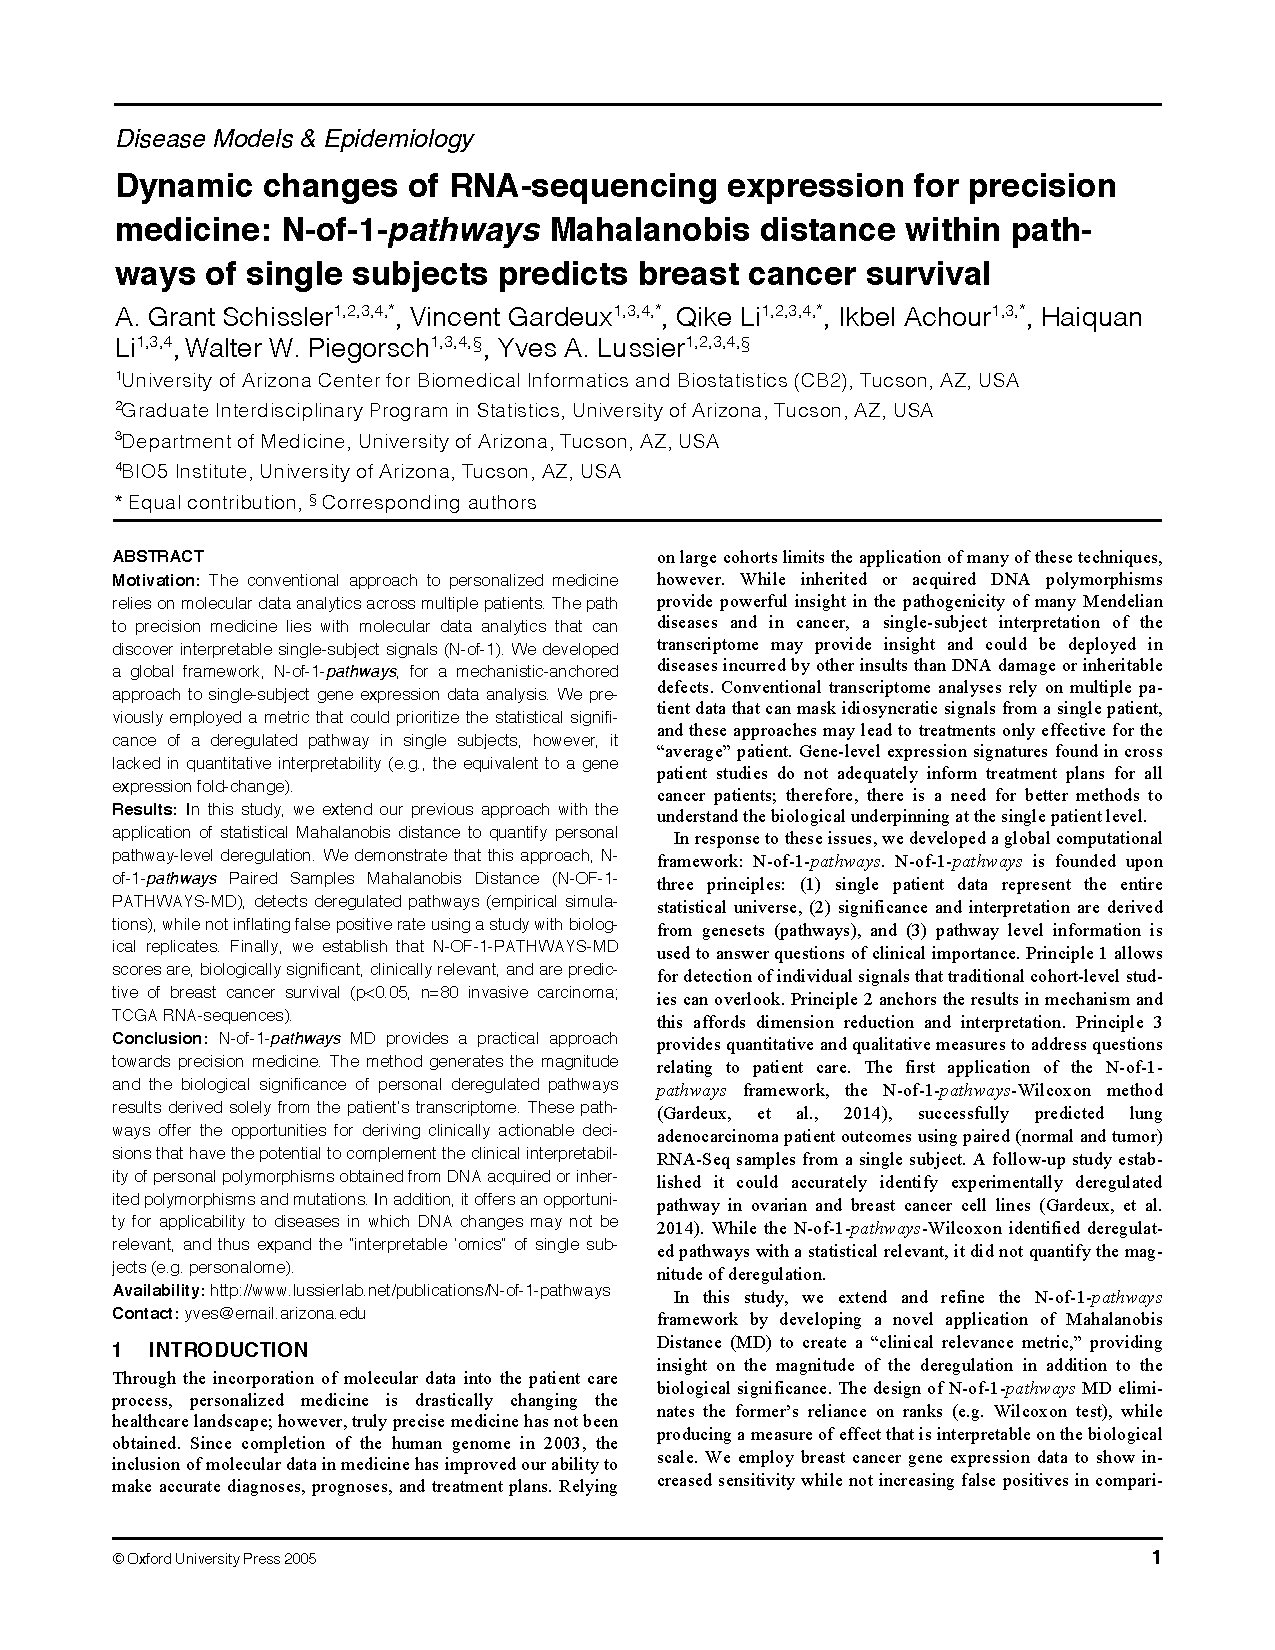
\includepdf[pages=-, scale=0.85, pagecommand={}]{md.pdf}
\renewcommand{\thetable}{B.\arabic{table}}
\chapter{Coverage rates for model specific BMDL and BMA BMDL}

\indent\indent Chapter \ref{Chap:Simu} illustrated the coverage rates for model specific BMDL and BMA BMDL via spaghetti plots (See Figures \ref{fig:SpaghettiM12M4}, \ref{fig:SpaghettiM52M8} and \ref{fig:BMABMDLCoverage}). Here, the actual values of coverage rates are provided supplement to those plots. Model codes are from Table \ref{dose_response}.

% latex table generated in R 3.0.2 by xtable 1.7-1 package
% Wed Dec 25 16:33:36 2013
\begin{table}[ht]
\caption{Coverage rates when fitting logistic model (M1) model to the simulated data generated by 8 models, under 5 configurations and 3 sample-sizes.}\label{cover1}
\renewcommand{\arraystretch}{1.25} %widens row widths
\vspace{8pt}
\centering
\scalebox{0.84}{
\begin{tabular}{lrrrrrrrrr}
  \hline
Configuration & $N$ & M1 & M2 & M3 & M4 & M5 & M6 & M7 & M8 \\
  \hline
C1 & 25 & 0.715 & 0.714 & 0.732 & 0.726 & 0.723 & 0.722 & 0.726 & 0.726 \\
& 50 & 0.791 & 0.797 & 0.807 & 0.801 & 0.798 & 0.810 & 0.803 & 0.801 \\
& 1000 & 0.937 & 0.953 & 0.989 & 0.969 & 0.973 & 0.979 & 0.987 & 0.978 \\
  \hline
  C2 & 25 & 0.773 & 0.753 & 0.482 & 0.868 & 0.820 & 0.817 & 0.817 & 0.820 \\
& 50 & 0.834 & 0.802 & 0.413 & 0.920 & 0.881 & 0.875 & 0.871 & 0.876 \\
& 1000 & 0.936 & 0.805 & 0.000 & 1.000 & 0.998 & 0.996 & 0.985 & 0.997 \\
  \hline
  C3 & 25 & 0.898 & 0.803 & 0.002 & 0.909 & 0.004 & 0.052 & 0.136 & 0.012 \\
& 50 & 0.917 & 0.770 & 0.000 & 0.929 & 0.000 & 0.002 & 0.020 & 0.000 \\
& 1000 & 0.954 & 0.065 & 0.000 & 0.979 & 0.000 & 0.000 & 0.000 & 0.000 \\
  \hline
  C4 & 25 & 0.877 & 0.873 & 0.203 & 0.999 & 0.936 & 0.990 & 0.998 & 0.976 \\
& 50 & 0.906 & 0.899 & 0.056 & 1.000 & 0.975 & 1.000 & 1.000 & 0.996 \\
& 1000 & 0.942 & 0.895 & 0.000 & 1.000 & 1.000 & 1.000 & 1.000 & 1.000 \\
  \hline
  C5 & 25 & 0.942 & 0.876 & 0.000 & 0.996 & 0.989 & 1.000 & 1.000 & 0.994 \\
& 50 & 0.940 & 0.841 & 0.000 & 0.999 & 0.994 & 1.000 & 1.000 & 0.998 \\
& 1000 & 0.952 & 0.213 & 0.000 & 1.000 & 1.000 & 1.000 & 1.000 & 1.000 \\
   \hline
\end{tabular}
}
\end{table}

% latex table generated in R 3.0.2 by xtable 1.7-1 package
% Wed Dec 25 16:33:36 2013
\begin{table}[ht]
\caption{Coverage rates when fitting probit model (M2) model to the simulated data generated by 8 models, under 5 configurations and 3 sample-sizes.}\label{cover1}
\renewcommand{\arraystretch}{1.25} %widens row widths
\vspace{8pt}
\centering
\scalebox{0.84}{
\begin{tabular}{lrrrrrrrrr}
  \hline
Configuration & $N$ & M1 & M2 & M3 & M4 & M5 & M6 & M7 & M8 \\
  \hline
C1 & 25 & 0.733 & 0.731 & 0.750 & 0.740 & 0.736 & 0.746 & 0.746 & 0.746 \\
& 50 & 0.799 & 0.803 & 0.815 & 0.811 & 0.811 & 0.812 & 0.815 & 0.815 \\
& 1000 & 0.915 & 0.936 & 0.988 & 0.953 & 0.962 & 0.973 & 0.981 & 0.972 \\
  \hline
  C2 & 25 & 0.815 & 0.796 & 0.566 & 0.897 & 0.847 & 0.846 & 0.849 & 0.851 \\
& 50 & 0.866 & 0.843 & 0.530 & 0.933 & 0.899 & 0.896 & 0.895 & 0.895 \\
& 1000 & 0.979 & 0.940 & 0.000 & 1.000 & 1.000 & 0.998 & 0.996 & 0.999 \\
  \hline
  C3 & 25 & 0.951 & 0.880 & 0.004 & 0.967 & 0.014 & 0.103 & 0.226 & 0.022 \\
& 50 & 0.979 & 0.908 & 0.000 & 0.983 & 0.000 & 0.011 & 0.065 & 0.000 \\
& 1000 & 1.000 & 0.952 & 0.000 & 1.000 & 0.000 & 0.000 & 0.000 & 0.000 \\
  \hline
  C4 & 25 & 0.885 & 0.880 & 0.164 & 0.998 & 0.942 & 0.991 & 0.997 & 0.979 \\
& 50 & 0.916 & 0.906 & 0.034 & 1.000 & 0.979 & 1.000 & 1.000 & 0.997 \\
& 1000 & 0.968 & 0.940 & 0.000 & 1.000 & 1.000 & 1.000 & 1.000 & 1.000 \\
  \hline
  C5 & 25 & 0.975 & 0.930 & 0.000 & 0.999 & 0.995 & 1.000 & 1.000 & 0.998 \\
& 50 & 0.983 & 0.940 & 0.000 & 1.000 & 0.999 & 1.000 & 1.000 & 0.999 \\
& 1000 & 1.000 & 0.942 & 0.000 & 1.000 & 1.000 & 1.000 & 1.000 & 1.000 \\
   \hline
\end{tabular}
}
\end{table}

% latex table generated in R 3.0.2 by xtable 1.7-1 package
% Wed Dec 25 16:33:36 2013
\begin{table}[ht]
\caption{Coverage rates when fitting quantal linear model (M3) model to the simulated data generated by 8 models, under 5 configurations and 3 sample-sizes.}\label{cover1}
\renewcommand{\arraystretch}{1.25} %widens row widths
\vspace{8pt}
\centering
\scalebox{0.84}{
\begin{tabular}{lrrrrrrrrr}
  \hline
Configuration & $N$ & M1 & M2 & M3 & M4 & M5 & M6 & M7 & M8 \\
  \hline
C1 & 25 & 0.724 & 0.736 & 0.827 & 0.723 & 0.769 & 0.764 & 0.749 & 0.764 \\
& 50 & 0.711 & 0.734 & 0.854 & 0.724 & 0.766 & 0.772 & 0.762 & 0.765 \\
& 1000 & 0.102 & 0.197 & 0.943 & 0.114 & 0.365 & 0.361 & 0.335 & 0.359 \\
  \hline
  C2 & 25 & 0.923 & 0.915 & 0.858 & 0.952 & 0.942 & 0.939 & 0.940 & 0.939 \\
& 50 & 0.940 & 0.941 & 0.877 & 0.966 & 0.956 & 0.954 & 0.952 & 0.955 \\
& 1000 & 1.000 & 1.000 & 0.946 & 1.000 & 1.000 & 1.000 & 1.000 & 1.000 \\
  \hline
  C3 & 25 & 0.999 & 0.998 & 0.911 & 0.999 & 0.940 & 0.977 & 0.989 & 0.953 \\
& 50 & 1.000 & 1.000 & 0.924 & 1.000 & 0.961 & 0.991 & 0.996 & 0.973 \\
& 1000 & 1.000 & 1.000 & 0.951 & 1.000 & 0.998 & 1.000 & 1.000 & 1.000 \\
  \hline
  C4 & 25 & 0.983 & 0.983 & 0.901 & 0.999 & 0.989 & 0.998 & 0.999 & 0.995 \\
& 50 & 0.999 & 0.999 & 0.923 & 1.000 & 1.000 & 1.000 & 1.000 & 1.000 \\
& 1000 & 1.000 & 1.000 & 0.946 & 1.000 & 1.000 & 1.000 & 1.000 & 1.000 \\
  \hline
  C5 & 25 & 1.000 & 1.000 & 0.929 & 1.000 & 1.000 & 1.000 & 1.000 & 1.000 \\
& 50 & 1.000 & 1.000 & 0.941 & 1.000 & 1.000 & 1.000 & 1.000 & 1.000 \\
& 1000 & 1.000 & 1.000 & 0.948 & 1.000 & 1.000 & 1.000 & 1.000 & 1.000 \\
   \hline
\end{tabular}
}
\end{table}
% latex table generated in R 3.0.2 by xtable 1.7-1 package
% Wed Dec 25 16:33:36 2013
\begin{table}[ht]
\caption{Coverage rates when fitting quantal quadratic model (M4) model to the simulated data generated by 8 models, under 5 configurations and 3 sample-sizes.}\label{cover1}
\renewcommand{\arraystretch}{1.25} %widens row widths
\vspace{8pt}
\centering
\scalebox{0.84}{
\begin{tabular}{lrrrrrrrrr}
  \hline
Configuration & $N$ & M1 & M2 & M3 & M4 & M5 & M6 & M7 & M8 \\
  \hline
C1 & 25 & 0.765 & 0.768 & 0.772 & 0.781 & 0.776 & 0.782 & 0.783 & 0.783 \\
& 50 & 0.825 & 0.827 & 0.828 & 0.831 & 0.831 & 0.840 & 0.839 & 0.837 \\
& 1000 & 0.897 & 0.936 & 0.991 & 0.944 & 0.969 & 0.978 & 0.984 & 0.975 \\
  \hline
  C2 & 25 & 0.656 & 0.607 & 0.263 & 0.809 & 0.726 & 0.723 & 0.705 & 0.726 \\
& 50 & 0.663 & 0.595 & 0.084 & 0.861 & 0.770 & 0.763 & 0.757 & 0.768 \\
& 1000 & 0.009 & 0.000 & 0.000 & 0.940 & 0.258 & 0.207 & 0.167 & 0.235 \\
  \hline
  C3 & 25 & 0.897 & 0.731 & 0.000 & 0.919 & 0.000 & 0.000 & 0.002 & 0.000 \\
& 50 & 0.903 & 0.625 & 0.000 & 0.933 & 0.000 & 0.000 & 0.000 & 0.000 \\
& 1000 & 0.760 & 0.000 & 0.000 & 0.958 & 0.000 & 0.000 & 0.000 & 0.000 \\
  \hline
  C4 & 25 & 0.003 & 0.002 & 0.000 & 0.912 & 0.018 & 0.434 & 0.621 & 0.109 \\
& 50 & 0.000 & 0.000 & 0.000 & 0.931 & 0.000 & 0.227 & 0.465 & 0.010 \\
& 1000 & 0.000 & 0.000 & 0.000 & 0.945 & 0.000 & 0.000 & 0.000 & 0.000 \\
  \hline
  C5 & 25 & 0.274 & 0.102 & 0.000 & 0.942 & 0.679 & 1.000 & 1.000 & 0.825 \\
& 50 & 0.070 & 0.004 & 0.000 & 0.948 & 0.523 & 1.000 & 1.000 & 0.767 \\
& 1000 & 0.000 & 0.000 & 0.000 & 0.952 & 0.000 & 1.000 & 1.000 & 0.019 \\
   \hline
\end{tabular}
}
\end{table}
% latex table generated in R 3.0.2 by xtable 1.7-1 package
% Wed Dec 25 16:33:36 2013
\begin{table}[ht]
\caption{Coverage rates when fitting two-stage model (M5) model to the simulated data generated by 8 models, under 5 configurations and 3 sample-sizes.}\label{cover1}
\renewcommand{\arraystretch}{1.25} %widens row widths
\vspace{8pt}
\centering
\scalebox{0.84}{
\begin{tabular}{lrrrrrrrrr}
  \hline
Configuration & $N$ & M1 & M2 & M3 & M4 & M5 & M6 & M7 & M8 \\
  \hline
C1 & 25 & 0.914 & 0.918 & 0.941 & 0.918 & 0.928 & 0.927 & 0.925 & 0.927 \\
& 50 & 0.890 & 0.898 & 0.954 & 0.894 & 0.917 & 0.919 & 0.923 & 0.916 \\
& 1000 & 0.839 & 0.883 & 0.986 & 0.904 & 0.930 & 0.942 & 0.959 & 0.938 \\
  \hline
  C2 & 25 & 0.932 & 0.928 & 0.950 & 0.924 & 0.931 & 0.933 & 0.942 & 0.927 \\
& 50 & 0.949 & 0.950 & 0.953 & 0.945 & 0.947 & 0.952 & 0.945 & 0.951 \\
& 1000 & 0.987 & 0.980 & 0.794 & 1.000 & 0.991 & 0.987 & 0.977 & 0.988 \\
  \hline
  C3 & 25 & 1.000 & 0.999 & 0.738 & 1.000 & 0.819 & 0.939 & 0.979 & 0.857 \\
& 50 & 1.000 & 1.000 & 0.702 & 1.000 & 0.797 & 0.938 & 0.981 & 0.842 \\
& 1000 & 1.000 & 0.974 & 0.721 & 1.000 & 0.912 & 0.993 & 1.000 & 0.962 \\
  \hline
  C4 & 25 & 0.983 & 0.982 & 0.725 & 0.999 & 0.994 & 1.000 & 1.000 & 0.999 \\
& 50 & 0.982 & 0.980 & 0.662 & 1.000 & 0.995 & 1.000 & 1.000 & 1.000 \\
& 1000 & 0.948 & 0.941 & 0.683 & 1.000 & 0.952 & 1.000 & 1.000 & 0.988 \\
  \hline
  C5 & 25 & 1.000 & 1.000 & 0.616 & 1.000 & 1.000 & 1.000 & 1.000 & 1.000 \\
& 50 & 1.000 & 0.999 & 0.634 & 1.000 & 1.000 & 1.000 & 1.000 & 1.000 \\
& 1000 & 0.818 & 0.684 & 0.722 & 1.000 & 0.990 & 1.000 & 1.000 & 0.999 \\
   \hline
\end{tabular}
}
\end{table}
% latex table generated in R 3.0.2 by xtable 1.7-1 package
% Wed Dec 25 16:33:36 2013
\begin{table}[ht]
\caption{Coverage rates when fitting log-logistic model (M6) model to the simulated data generated by 8 models, under 5 configurations and 3 sample-sizes.}\label{cover1}
\renewcommand{\arraystretch}{1.25} %widens row widths
\vspace{8pt}
\centering
\scalebox{0.84}{
\begin{tabular}{lrrrrrrrrr}
  \hline
Configuration & $N$ & M1 & M2 & M3 & M4 & M5 & M6 & M7 & M8 \\
  \hline
C1 & 25 & 0.738 & 0.732 & 0.801 & 0.751 & 0.754 & 0.756 & 0.759 & 0.757 \\
& 50 & 0.711 & 0.713 & 0.767 & 0.725 & 0.722 & 0.733 & 0.721 & 0.742 \\
& 1000 & 0.878 & 0.882 & 0.922 & 0.927 & 0.909 & 0.929 & 0.946 & 0.926 \\
  \hline
  C2 & 25 & 0.996 & 0.997 & 0.995 & 0.998 & 0.998 & 0.996 & 0.999 & 0.998 \\
& 50 & 0.995 & 0.992 & 0.989 & 0.994 & 0.995 & 0.992 & 0.994 & 0.995 \\
& 1000 & 0.975 & 0.975 & 0.970 & 0.960 & 0.971 & 0.963 & 0.940 & 0.966 \\
  \hline
  C3 & 25 & 0.969 & 0.966 & 0.973 & 0.973 & 0.969 & 0.973 & 0.981 & 0.967 \\
& 50 & 0.947 & 0.948 & 0.958 & 0.954 & 0.955 & 0.966 & 0.977 & 0.957 \\
& 1000 & 0.905 & 0.879 & 0.870 & 0.931 & 0.835 & 0.954 & 0.980 & 0.878 \\
  \hline
  C4 & 25 & 0.964 & 0.961 & 0.968 & 0.980 & 0.965 & 0.984 & 0.985 & 0.971 \\
& 50 & 0.930 & 0.930 & 0.954 & 0.951 & 0.930 & 0.973 & 0.979 & 0.951 \\
& 1000 & 0.545 & 0.507 & 0.720 & 0.825 & 0.553 & 0.948 & 0.986 & 0.785 \\
  \hline
  C5 & 25 & 0.785 & 0.754 & 0.901 & 0.850 & 0.829 & 0.951 & 0.961 & 0.845 \\
& 50 & 0.639 & 0.607 & 0.814 & 0.788 & 0.749 & 0.956 & 0.964 & 0.786 \\
& 1000 & 0.000 & 0.000 & 0.000 & 0.051 & 0.008 & 0.962 & 0.957 & 0.042 \\
   \hline
\end{tabular}
}
\end{table}

% latex table generated in R 3.0.2 by xtable 1.7-1 package
% Wed Dec 25 16:33:36 2013
\begin{table}[ht]
\caption{Coverage rates when fitting log-probit model (M7) model to the simulated data generated by 8 models, under 5 configurations and 3 sample-sizes.}\label{cover1}
\renewcommand{\arraystretch}{1.25} %widens row widths
\vspace{8pt}
\centering
\scalebox{0.84}{
\begin{tabular}{lrrrrrrrrr}
  \hline
Configuration & $N$ & M1 & M2 & M3 & M4 & M5 & M6 & M7 & M8 \\
  \hline
C1 & 25 & 0.735 & 0.739 & 0.814 & 0.738 & 0.756 & 0.764 & 0.771 & 0.765 \\
& 50 & 0.713 & 0.724 & 0.763 & 0.724 & 0.732 & 0.732 & 0.727 & 0.737 \\
& 1000 & 0.833 & 0.846 & 0.900 & 0.896 & 0.875 & 0.897 & 0.923 & 0.895 \\
  \hline
  C2 & 25 & 0.999 & 0.998 & 0.995 & 0.998 & 0.997 & 0.998 & 0.998 & 0.997 \\
& 50 & 0.994 & 0.992 & 0.989 & 0.994 & 0.995 & 0.994 & 0.993 & 0.995 \\
& 1000 & 0.978 & 0.981 & 0.974 & 0.970 & 0.977 & 0.970 & 0.956 & 0.971 \\
  \hline
  C3 & 25 & 0.964 & 0.962 & 0.964 & 0.969 & 0.961 & 0.967 & 0.976 & 0.962 \\
& 50 & 0.940 & 0.936 & 0.949 & 0.948 & 0.942 & 0.960 & 0.969 & 0.942 \\
& 1000 & 0.884 & 0.872 & 0.718 & 0.914 & 0.683 & 0.902 & 0.954 & 0.739 \\
  \hline
  C4 & 25 & 0.957 & 0.957 & 0.965 & 0.973 & 0.959 & 0.981 & 0.983 & 0.968 \\
& 50 & 0.914 & 0.910 & 0.945 & 0.940 & 0.915 & 0.963 & 0.971 & 0.942 \\
& 1000 & 0.376 & 0.338 & 0.532 & 0.701 & 0.411 & 0.904 & 0.954 & 0.671 \\
  \hline
  C5 & 25 & 0.757 & 0.733 & 0.891 & 0.839 & 0.811 & 0.949 & 0.960 & 0.832 \\
& 50 & 0.606 & 0.570 & 0.788 & 0.769 & 0.723 & 0.949 & 0.963 & 0.768 \\
& 1000 & 0.000 & 0.000 & 0.000 & 0.046 & 0.004 & 0.954 & 0.948 & 0.022 \\
   \hline
\end{tabular}
}
\end{table}

% latex table generated in R 3.0.2 by xtable 1.7-1 package
% Wed Dec 25 16:33:36 2013
\begin{table}[ht]
\caption{Coverage rates when fitting Weibull model (M8) model to the simulated data generated by 8 models, under 5 configurations and 3 sample-sizes.}\label{cover1}
\renewcommand{\arraystretch}{1.25} %widens row widths
\vspace{8pt}
\centering
  \scalebox{0.84}{
\begin{tabular}{lrrrrrrrrr}
  \hline
Configuration & $N$ & M1 & M2 & M3 & M4 & M5 & M6 & M7 & M8 \\
  \hline
C1 & 25 & 0.949 & 0.960 & 0.972 & 0.965 & 0.967 & 0.968 & 0.965 & 0.969 \\
& 50 & 0.924 & 0.928 & 0.966 & 0.932 & 0.942 & 0.948 & 0.949 & 0.943 \\
& 1000 & 0.884 & 0.892 & 0.985 & 0.934 & 0.927 & 0.942 & 0.957 & 0.938 \\
  \hline
  C2 & 25 & 0.944 & 0.935 & 0.889 & 0.962 & 0.951 & 0.949 & 0.956 & 0.953 \\
& 50 & 0.956 & 0.941 & 0.858 & 0.973 & 0.966 & 0.965 & 0.959 & 0.965 \\
& 1000 & 0.973 & 0.967 & 0.803 & 0.954 & 0.967 & 0.957 & 0.930 & 0.962 \\
  \hline
  C3 & 25 & 0.963 & 0.953 & 0.649 & 0.966 & 0.720 & 0.860 & 0.914 & 0.764 \\
& 50 & 0.954 & 0.945 & 0.656 & 0.958 & 0.740 & 0.896 & 0.951 & 0.788 \\
& 1000 & 0.940 & 0.922 & 0.671 & 0.952 & 0.885 & 0.984 & 0.996 & 0.942 \\
  \hline
  C4 & 25 & 0.882 & 0.876 & 0.601 & 0.989 & 0.918 & 0.985 & 0.991 & 0.959 \\
& 50 & 0.891 & 0.882 & 0.597 & 0.972 & 0.920 & 0.982 & 0.990 & 0.957 \\
& 1000 & 0.868 & 0.843 & 0.598 & 0.956 & 0.862 & 0.994 & 0.999 & 0.953 \\
  \hline
  C5 & 25 & 0.899 & 0.880 & 0.528 & 0.950 & 0.938 & 0.994 & 0.993 & 0.948 \\
& 50 & 0.878 & 0.848 & 0.529 & 0.949 & 0.933 & 0.997 & 0.997 & 0.952 \\
& 1000 & 0.354 & 0.147 & 0.556 & 0.954 & 0.863 & 1.000 & 1.000 & 0.954 \\
   \hline
\end{tabular}
}
\end{table}

% latex table generated in R 3.0.2 by xtable 1.7-1 package
% Wed Dec 25 16:33:36 2013
\begin{table}[ht]
\caption{Coverage rates when applying Bayesian model averaging to the simulated data generated by 8 models, under 5 configurations and 3 sample-sizes.}\label{cover1}
\renewcommand{\arraystretch}{1.25} %widens row widths
\vspace{8pt}
\centering
  \scalebox{0.84}{
\begin{tabular}{lrrrrrrrrr}
  \hline
Configuration & $N$ & M1 & M2 & M3 & M4 & M5 & M6 & M7 & M8 \\
  \hline
C1 & 25 & 0.753 & 0.754 & 0.786 & 0.755 & 0.765 & 0.769 & 0.767 & 0.769 \\
& 50 & 0.804 & 0.808 & 0.844 & 0.817 & 0.820 & 0.823 & 0.827 & 0.825 \\
& 1000 & 0.909 & 0.924 & 0.967 & 0.948 & 0.936 & 0.952 & 0.964 & 0.950 \\
  \hline
  C2 & 25 & 0.901 & 0.895 & 0.838 & 0.933 & 0.916 & 0.914 & 0.917 & 0.917 \\
& 50 & 0.924 & 0.918 & 0.869 & 0.950 & 0.933 & 0.937 & 0.931 & 0.935 \\
& 1000 & 0.982 & 0.974 & 0.902 & 0.988 & 0.979 & 0.972 & 0.942 & 0.974 \\
  \hline
  C3 & 25 & 0.990 & 0.982 & 0.940 & 0.991 & 0.938 & 0.960 & 0.971 & 0.942 \\
& 50 & 0.989 & 0.973 & 0.923 & 0.993 & 0.927 & 0.955 & 0.970 & 0.935 \\
& 1000 & 0.989 & 0.895 & 0.951 & 0.992 & 0.984 & 0.985 & 0.990 & 0.984 \\
  \hline
  C4 & 25 & 0.976 & 0.975 & 0.930 & 0.998 & 0.983 & 0.997 & 1.000 & 0.989 \\
& 50 & 0.988 & 0.986 & 0.925 & 0.997 & 0.993 & 0.999 & 0.998 & 0.997 \\
& 1000 & 0.973 & 0.958 & 0.917 & 0.979 & 0.985 & 0.976 & 0.987 & 0.978 \\
  \hline
  C5 & 25 & 0.959 & 0.940 & 0.888 & 0.992 & 0.988 & 0.998 & 0.998 & 0.992 \\
& 50 & 0.960 & 0.910 & 0.900 & 0.994 & 0.992 & 1.000 & 0.999 & 0.995 \\
& 1000 & 0.974 & 0.876 & 0.922 & 0.988 & 0.974 & 0.968 & 0.957 & 0.956 \\
   \hline
\end{tabular}
}
\end{table} 
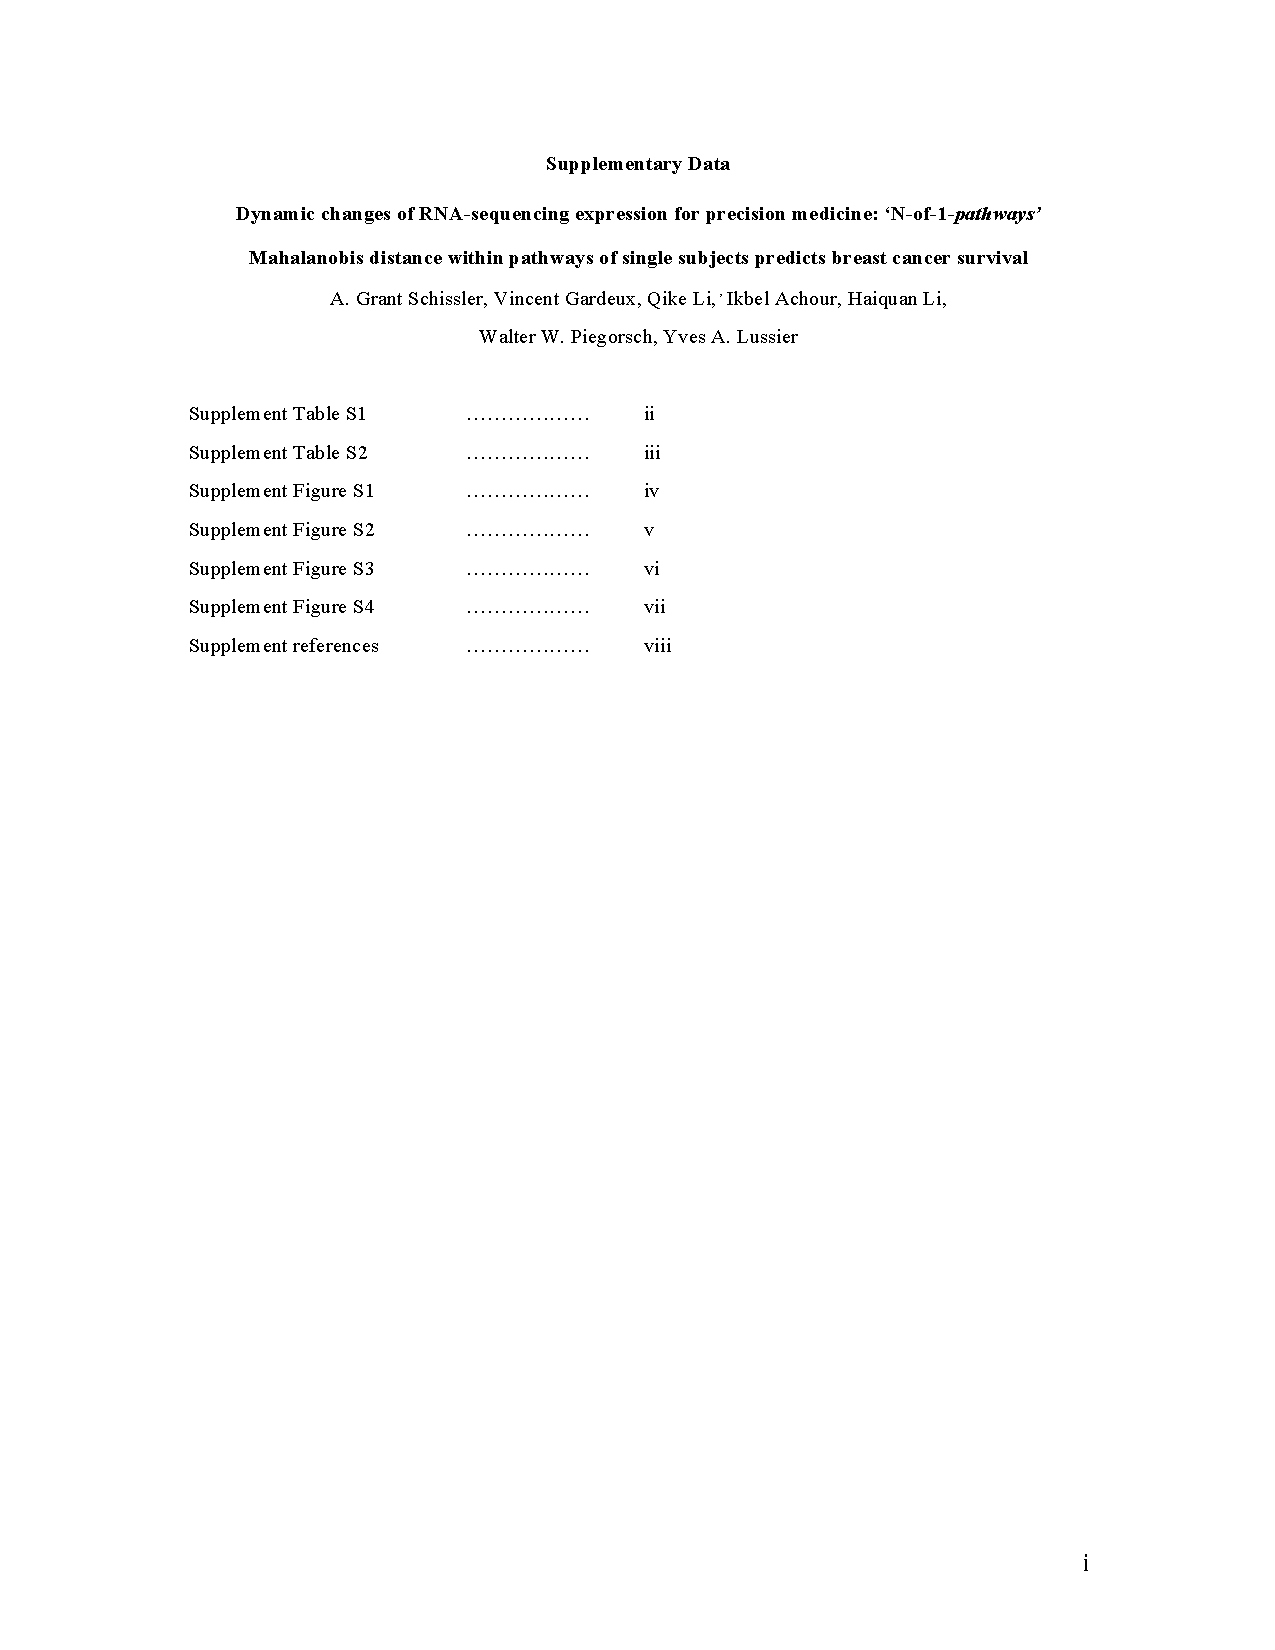
\includepdf[pages=-, scale=0.85, pagecommand={}]{md_supplement.pdf}
\renewcommand{\thetable}{C.\arabic{table}}
\chapter{Testing for differentially expressed genetic pathways with single-subject N-of-1 data in the presence of inter-gene correlation}\label{App:C}


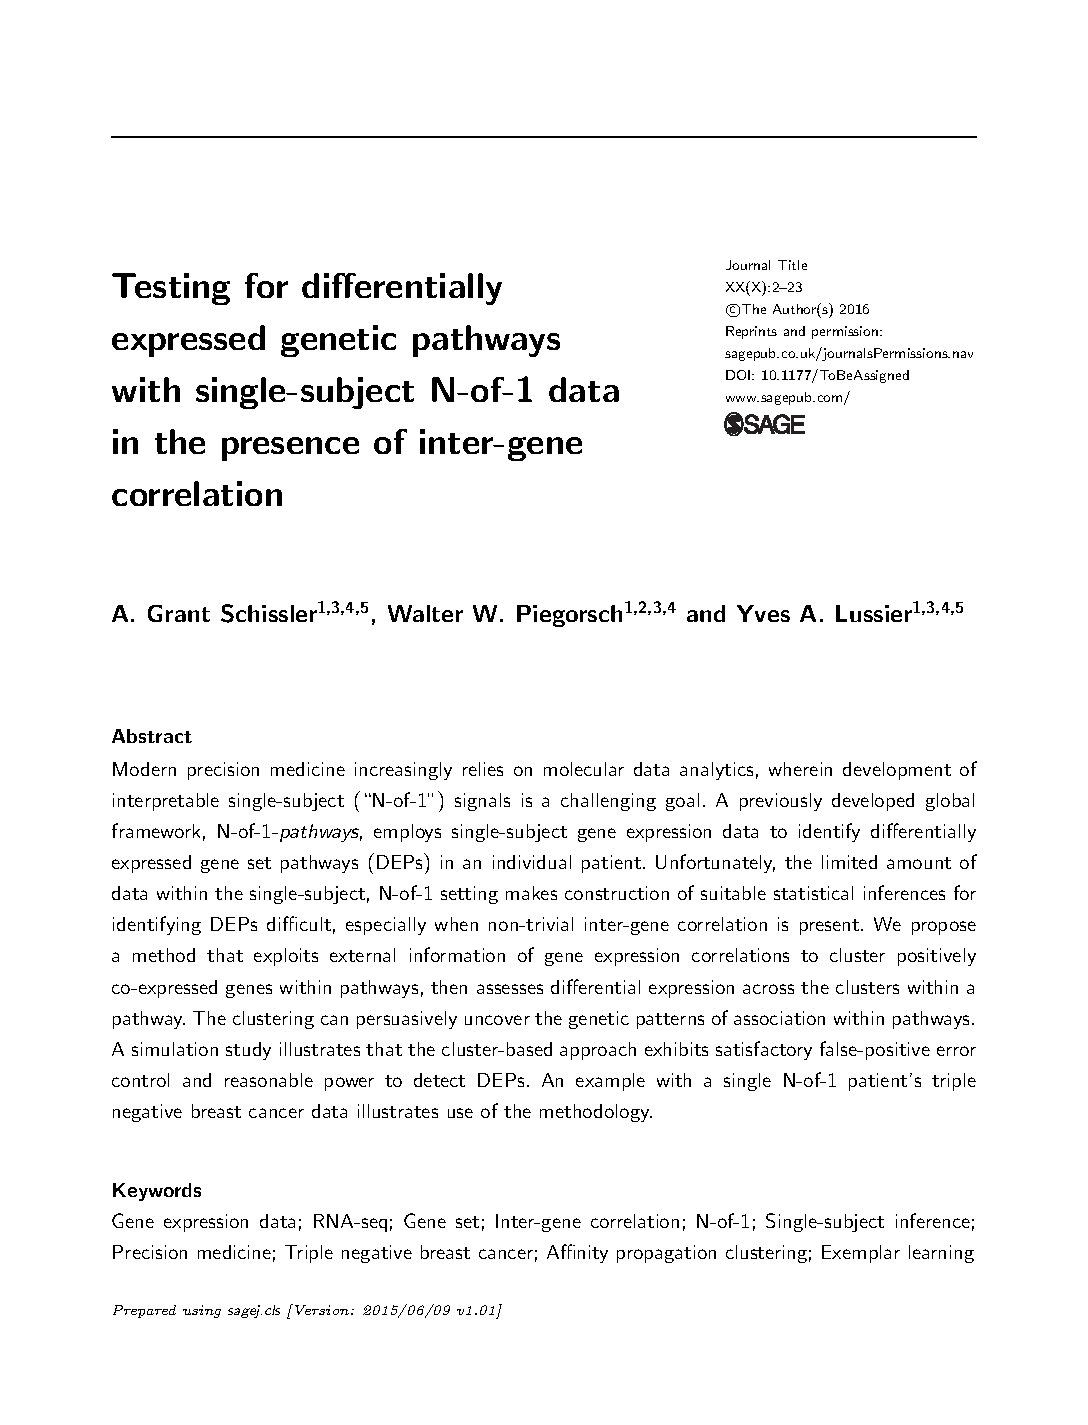
\includepdf[pages=-, scale=0.85, pagecommand={}]{clustered_T_smmr_v10.pdf}
\renewcommand{\thetable}{D.\arabic{table}}
\chapter{Supplementary material to Appendix C} \label{App:C}

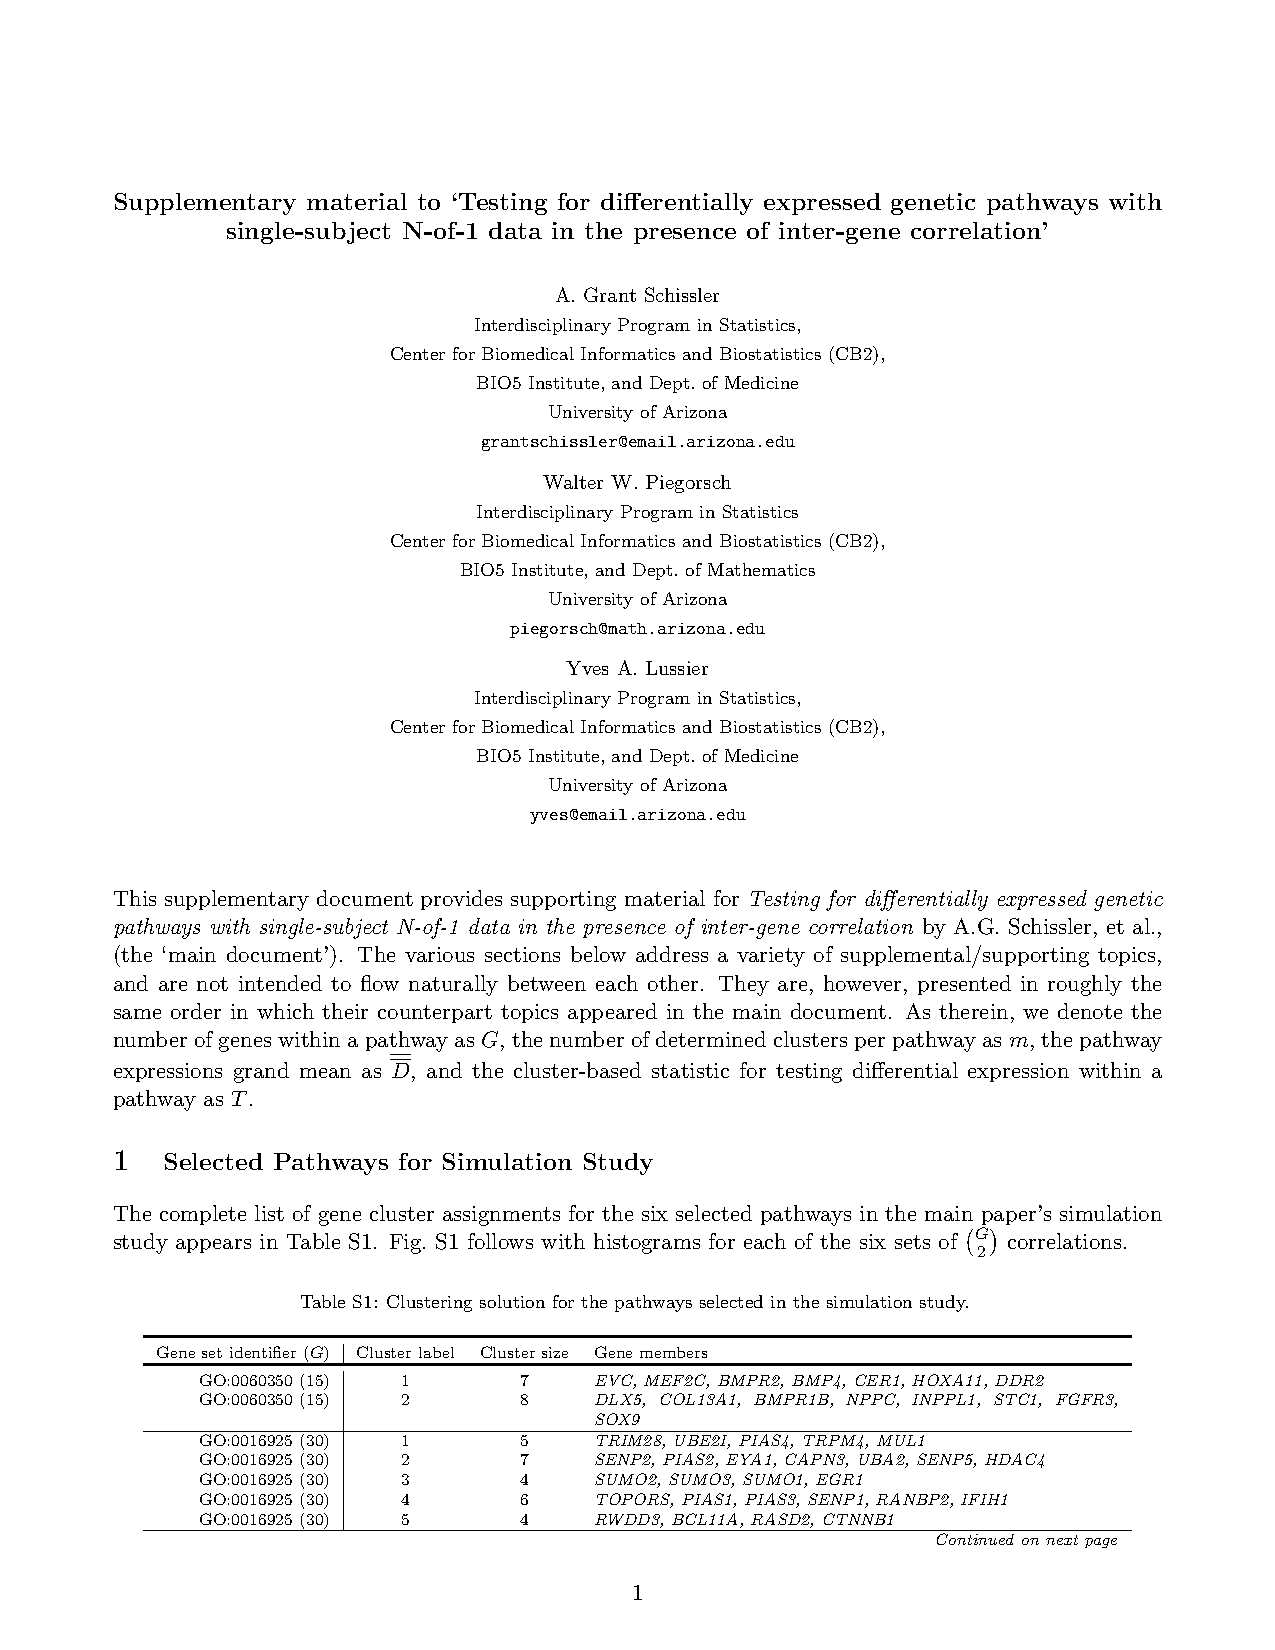
\includepdf[pages=-, scale=0.85, pagecommand={}]{clustered_T_suppl_v4.pdf}
\renewcommand{\thetable}{E.\arabic{table}}
\chapter{Analysis of aggregated cell-cell statistical distances within pathways unveils therapeutic-resistance mechanisms in circulating tumor cells}\label{App:E}


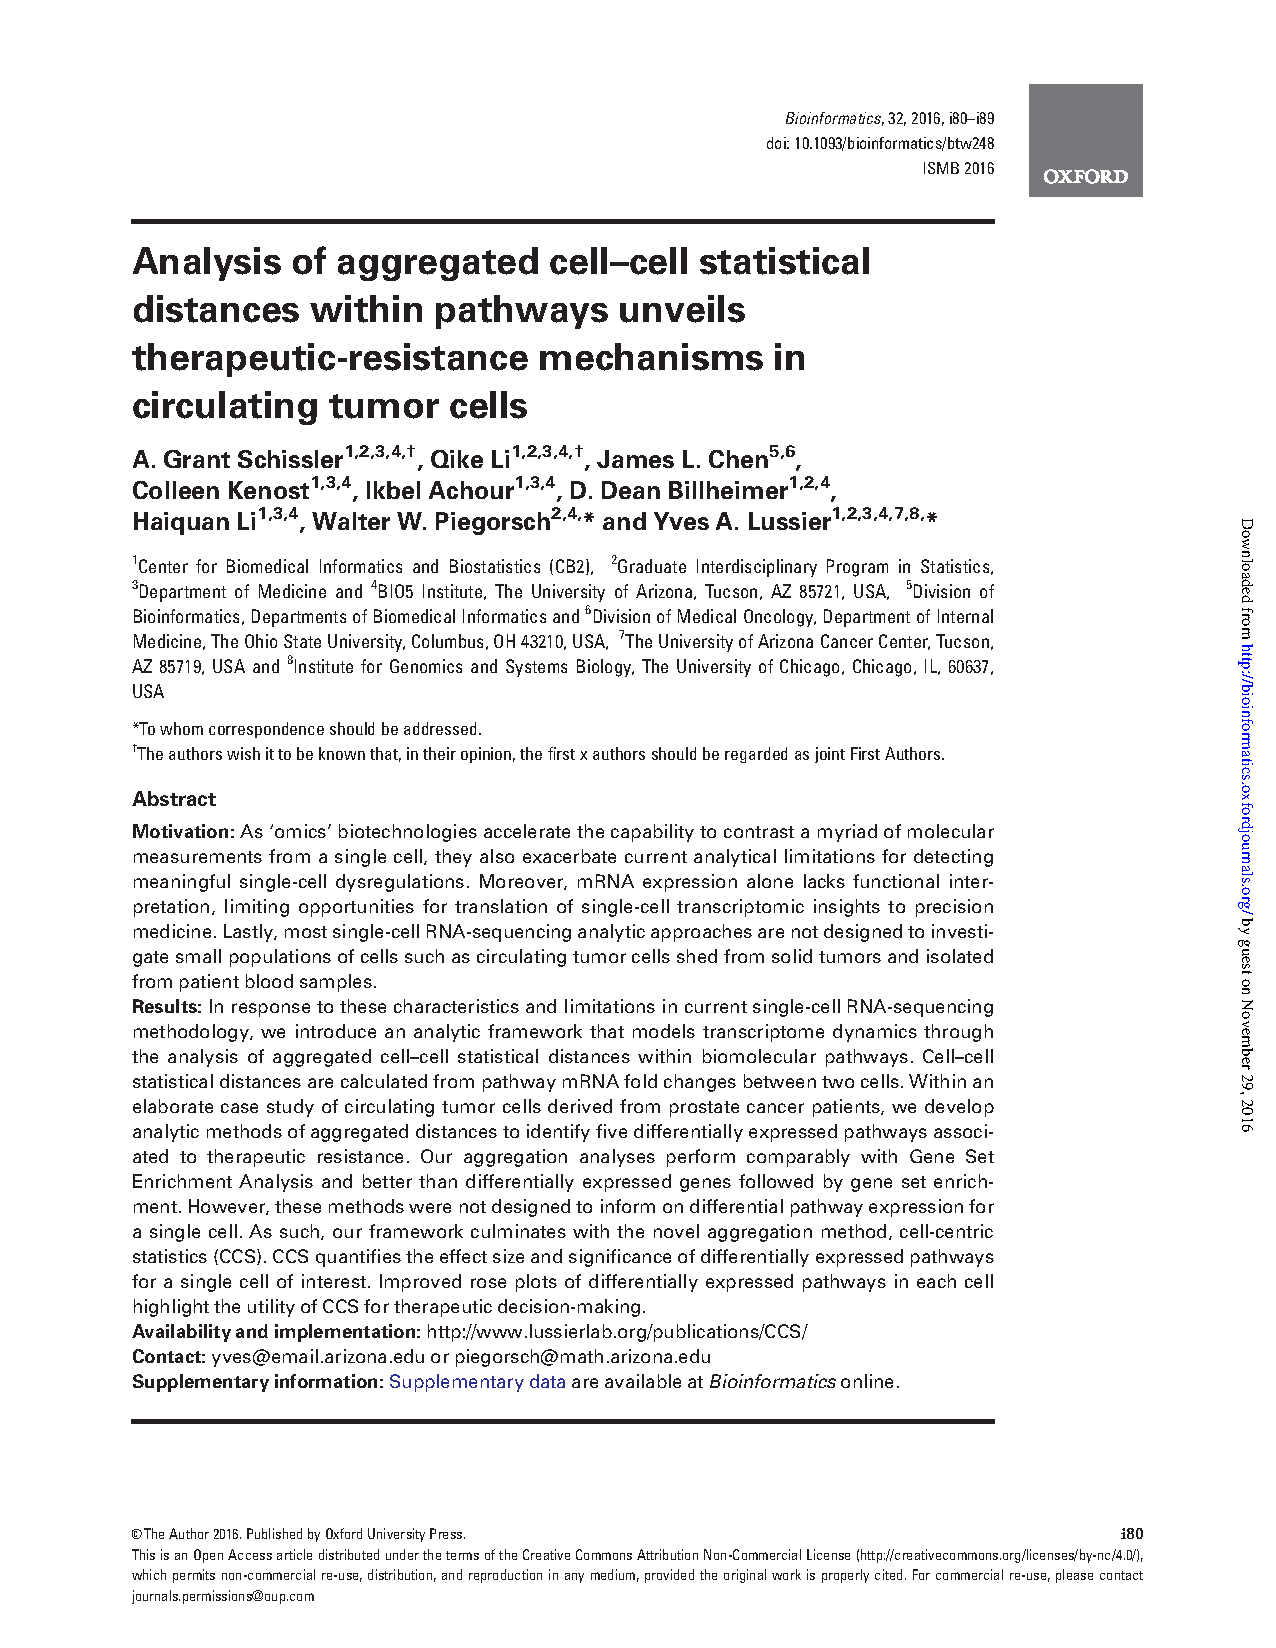
\includepdf[pages=-, scale=0.85, pagecommand={}]{ctcs.pdf}
\renewcommand{\thetable}{F.\arabic{table}}
% \chapter{Analysis of aggregated cell-cell statistical distances within pathways unveils therapeutic-resistance mechanisms in circulating tumor cells supplementary material}

\chapter{Supplementary material to Appendix E}


% 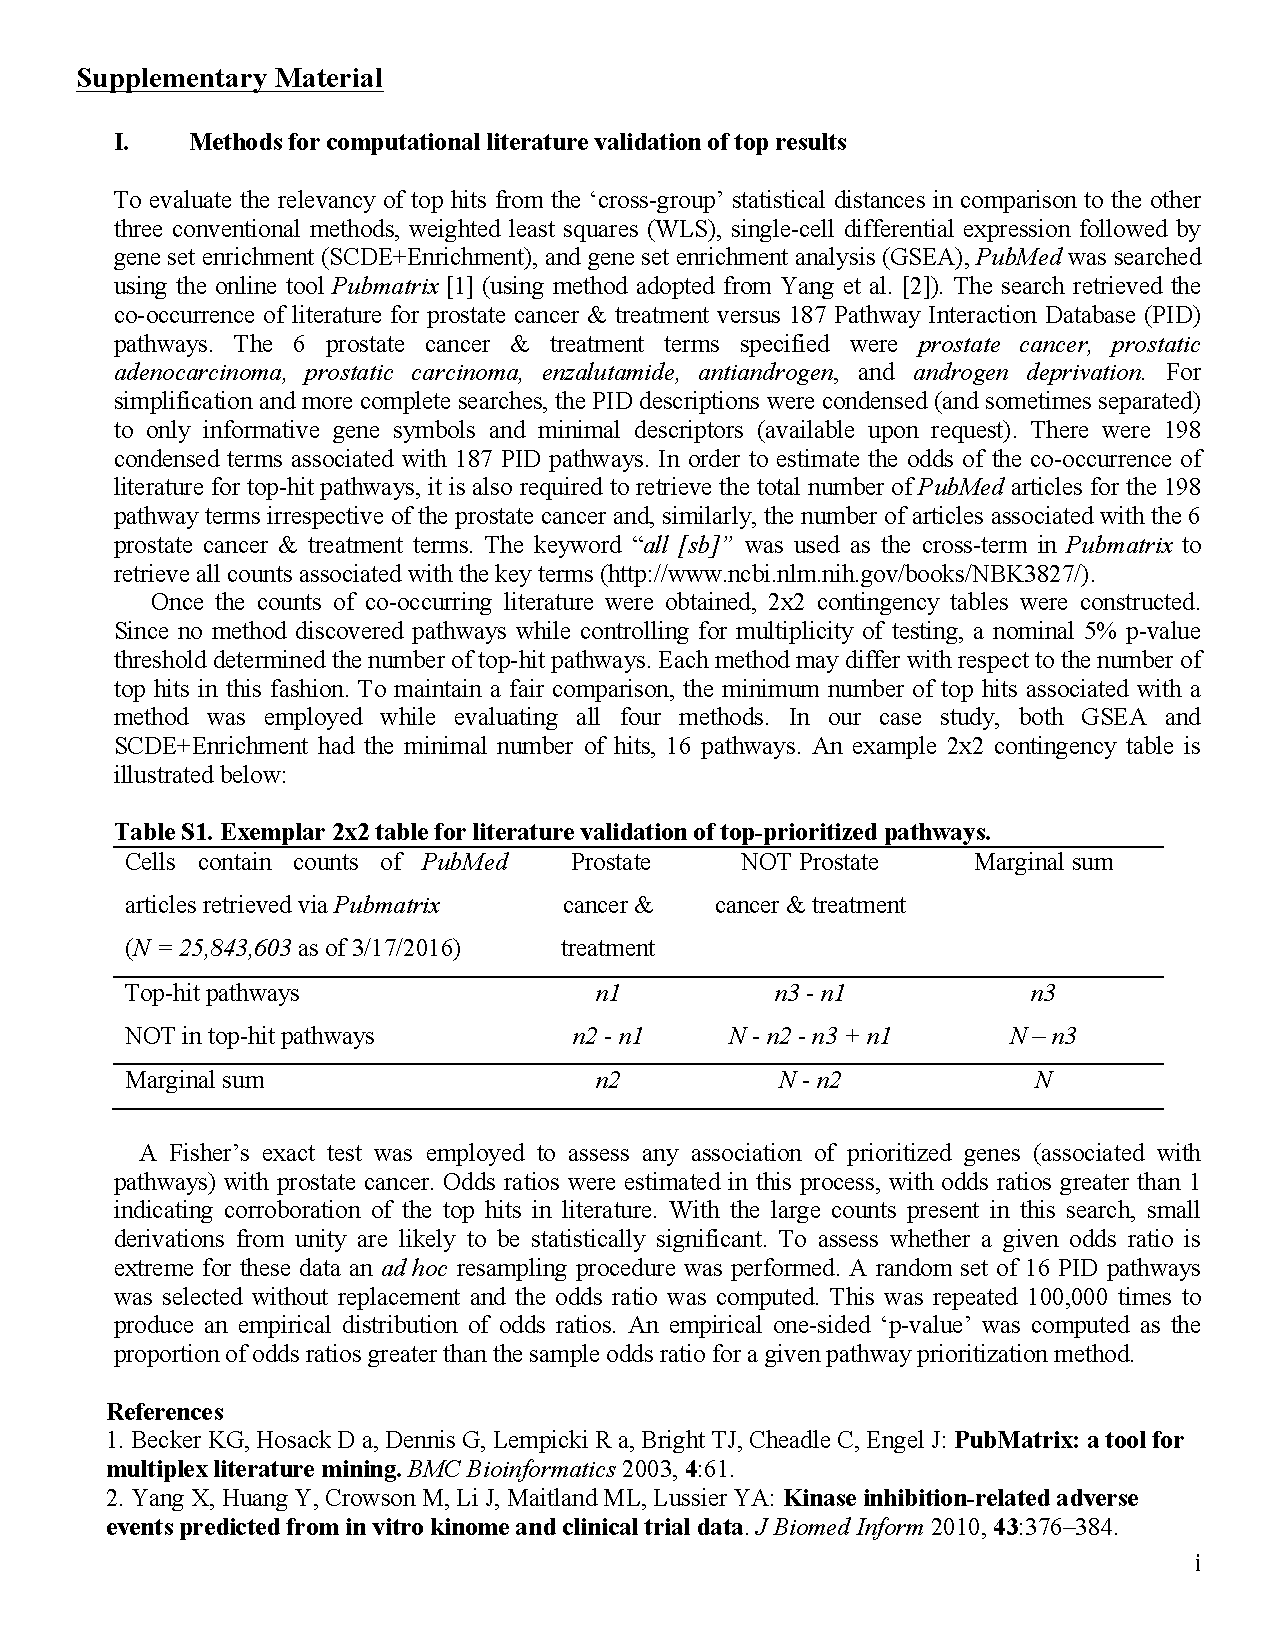
\includepdf[pages=-, offset=0 -25]{ctcs_supplment.pdf}
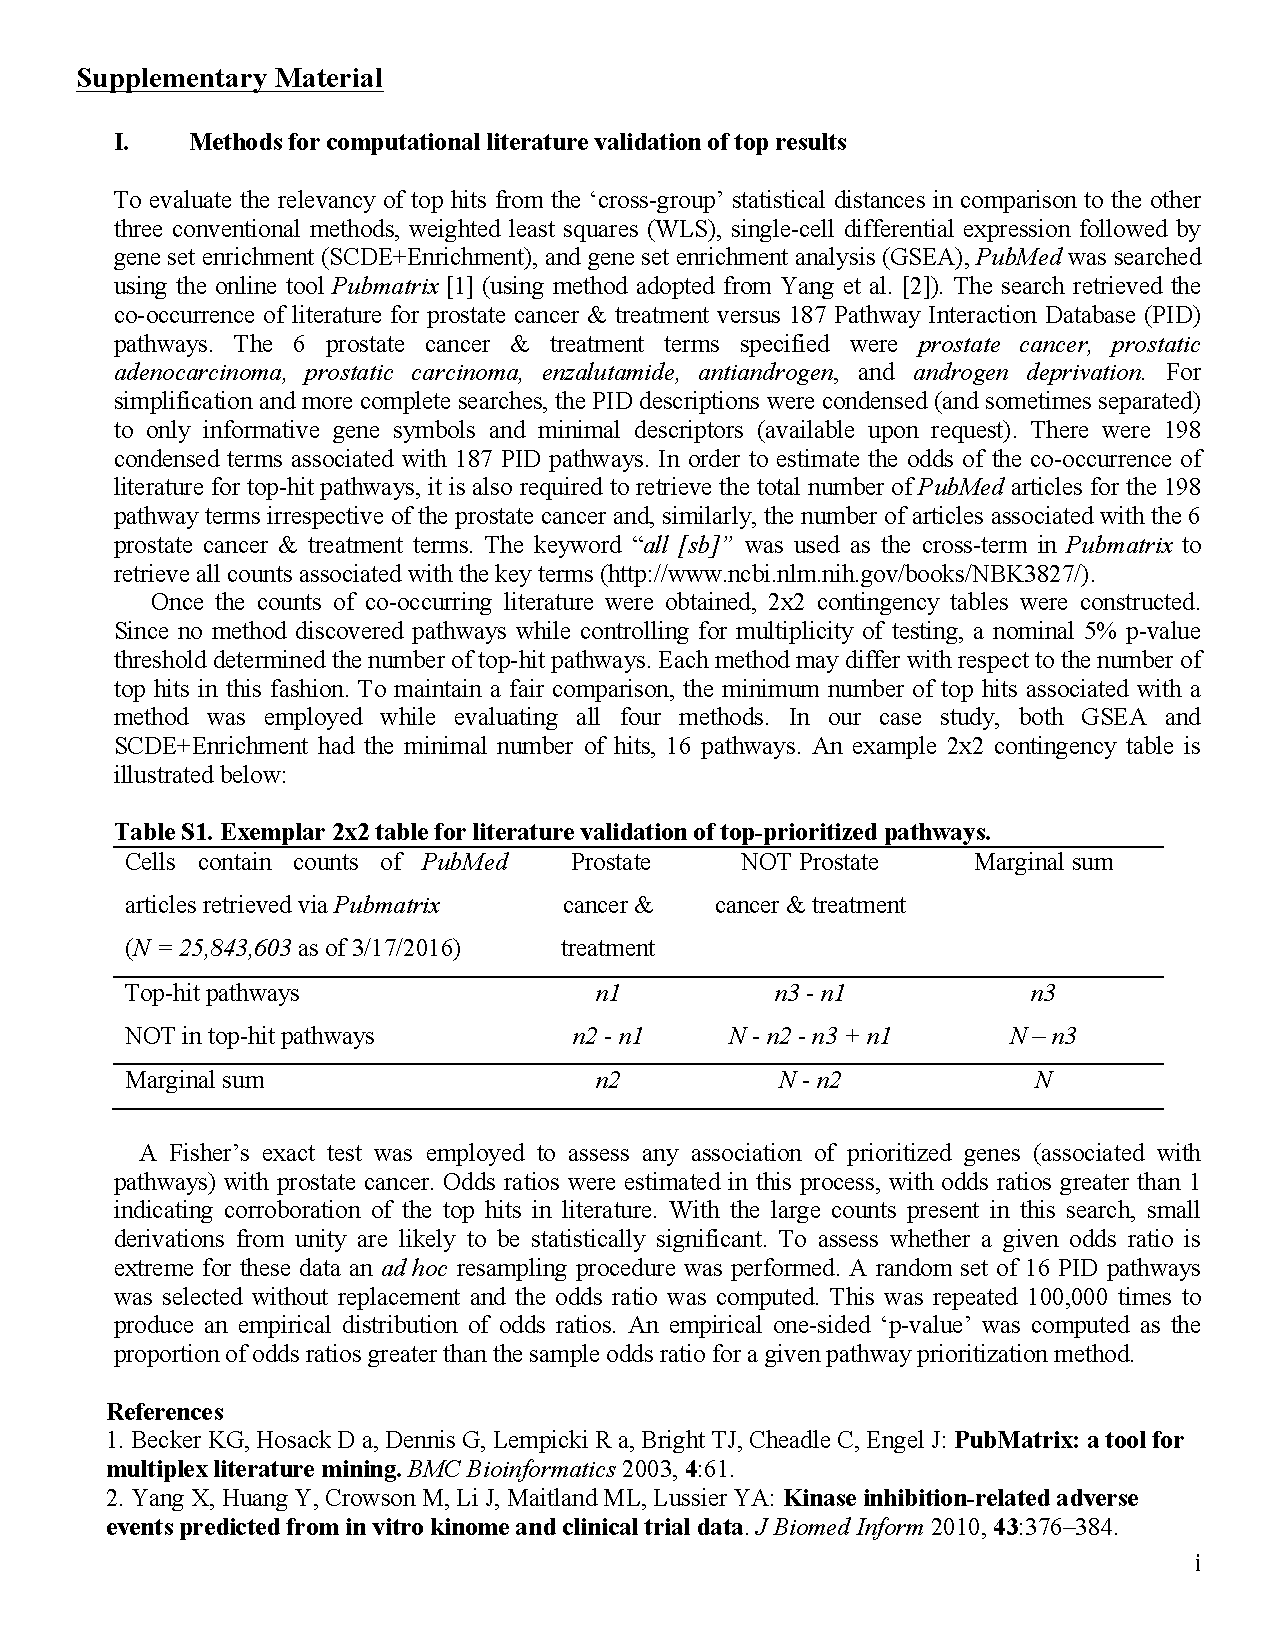
\includepdf[pages=-, scale=0.85, pagecommand={}]{ctcs_supplment.pdf}
%% unifying equations
\renewcommand{\thetable}{G.\arabic{table}}
\chapter{Unifying framework} \label{App:eqns}

\indent \indent A unifying theme of the three works contained in Appendices \ref{App:A} - \ref{App:F} is that of processes comparing the pathway-level mRNA expression derived from a single sample to one or more similarly structured samples. This Appendix provides a conceptual framework that subsumes the seemingly disparate approaches provided in the three articles. The framework below focuses on  development of an effect size and a P-value for describing and testing differential pathway expression of a single-sample versus one or more samples. This is not attempt at absolute rigor, but only to provide a generalization of common ideas throughout.

Consider a single baseline sample and denote its observed log-normalized expression as $B_{g}$ across the $g=1,2,\ldots,G$ total mRNAs in the transcriptome. Further, suppose there are $m$ case samples to be compared to the baseline sample. Denote the observed (log) expression in the $i^{th}$ case sample for the $g^{th}$ gene as $C_{ig}$ for $i=1,2,\ldots,m$. The core quantity of interest in differential expression is the difference
\begin{equation*}
\label{eq:diff}
D_{ig}=C_{ig}-B_{g}. \tag{1}
\end{equation*}

A key feature of the works contained in this dissertation is the integration of external knowledgebases into the statistical procedures. Indeed, pathways differ based on the annotations provided. Denote all information from external sources as $\Xi$. Suppose a given pathway of interest has $N$ mRNAs annotated from a knowledgebase (given by arbitrary external sources, $\Xi$). The approaches taken in Appendices \ref{App:A} - \ref{App:F} are so-called \lq self-contained\rq~gene set tests. This terminology refers to the fact that only the $N$ genes annotated to the pathway impact the effect size calculation and significance test procedure (i.e., the other mRNAs in the transcriptome are not considered). Denote the matrix of associated $N \times m$ gene-level differences comparing a single baseline sample against $m$ case samples for the pathway as
\begin{equation*}
  \label{eq:Dmat}
  \mathbf{D}_{\Xi} = \left ( \begin{array}{rcccc}
    D_{11} & D_{21} & \ldots & D_{m1} \\
    D_{12} & \ddots &  & \vdots \\
    \vdots &  & \ddots &  \\
    D_{1N} & \ldots &  & D_{mN} \\
\end{array} \right ) \tag{2}.
\end{equation*}

\noindent \noindent For simplicity of notation, we refer to $\mathbf{D}_{\Xi}$ as simply $\mathbf{D}$ below.

A critical feature in this setting is that the observations (the $N$ mRNAs) are not independent units. In fact, there are two types of dependencies to keep in mind: (i) the dependence between the samples as they are often derived from the same organism and (ii) the co-expression of mRNAs due to a multitude of biological factors (i.e., systems biology). To generalize the impact of inter-observation correlation, let $\Psi(\mathbf{D}; \Xi)$ denote some arbitrary parameter relating to these two types of dependencies (the inclusion of $\Xi$ is to remind the reader of the importance of knowledgebase information into this self-contained test).

In each article (Appendices \ref{App:A} - \ref{App:F}), there is an attempt to first summarize the central tendency of the gene-level expression differences. Denote an arbitrary parameter that quantifies differential expression while accounting for inter-observation correlation as $\theta$.

Ideally, $\theta$ also provides a context-relevant interpretation (an effect size). In Appendix \ref{App:A}, $\theta$ is the expected value of a transformed vector of observed differences, $D_{ig}$ with $m=1$. The transformation results from the adoption of the Mahalanobis distance (MD). The expected value is estimated via averaging the adjusted $D_{ig}$\rq s. We refer to this estimator as $\hat{\theta}(\mathbf{D}, \Psi)$. In that construction, the inter-observation adjustment accounts for the between-sample correlation structure (but not the inter-gene correlation). The observed average MD distance within the pathway, $\hat{\theta}(\mathbf{D}, \Psi)$, can be interpreted as an adjusted pathway-level fold-change in gene expression and was seen to be a clinically relevant metric (refer to Appendix \ref{App:A}). In Appendix \ref{App:C}, again an effect size is constructed in the $m=1$ scenario. However, $\hat{\theta}(\mathbf{D}, \Psi)$ in this article is simply the unadjusted average of the observed $D_{ig}$\rq s and interpreted as the average log fold-change in gene expression. In Appendix \ref{App:E}, both $\theta$ and $\hat{\theta}(\mathbf{D}, \Psi)$ are more complex. $\theta$ is no longer an expected value, but an overall measure of differential pathway expression across $m$ sample pairings. First, the $\mathbf{D}$ matrix is transformed into a $m$-dimensional vector containing the corresponding average MDs, one MD for each case sample. Then the median of average MDs is selected to provide $\hat{\theta}(\mathbf{D}, \Psi)$, an estimate of the overall differential pathway expression between the baseline sample and $m$ case samples.

With an effect size of differential expression in hand, the next task is to assess variation of the $\hat{\theta}(\mathbf{D}, \Psi)$ statistic. Denote a general parameter measuring variation of $\hat{\theta}(\mathbf{D}, \Psi)$ as $\phi$.

%\begin{equation}
%\label{eq:var}
%\phi(\hat{\theta};~\mathbf{D},\Psi). \tag{1}
%\end{equation}

$\phi$ was estimated by employing a variety of techniques within the respective articles. In Appendix \ref{App:A}, $\phi$ was estimated via a nonparametric bootstrapping procedure. This estimation was enhanced in Appendix \ref{App:C} via a cluster-correlated variance estimator by greater inclusion of the external sources contained with $\Xi$. In fact, $\Psi$ in Appendix \ref{App:C} now accounts for inter-gene correlation, not simply correlation between the paired samples. In Appendix \ref{App:E}, $\phi$ was estimated in exactly the same manner as in Appendix \ref{App:A} after the median pair was selected in the estimation of $\theta$.

Next, a test statistic is constructed to with an aim to subsequently estimate the probability that the pathway is differentially expressed for a baseline sample compared to $m$ case samples. Specifically, the following pair of hypotheses are tested:
\begin{equation}
  \label{eq:hypotheses}
\begin{array}{rl} \tag{3}
  H_{0}: & \theta = 0. \\
  H_{1}: & \theta \neq 0.
\end{array}
\end{equation}

\noindent \noindent Denote this test statistic under the null hypothesis in Equation (\ref{eq:hypotheses}) as
\begin{equation}
\label{eq:testStat}
t(\hat{\theta},\hat{\phi};~\mathbf{D},\Psi,\Xi). \tag{4}
\end{equation}

Finally, each work seeks to provide a P-value estimating the probability that the null hypothesis $H_{0}$ is true. In Appendix \ref{App:A}, this is accomplished via nonparametric bootstrapping of $\hat{\theta}(\mathbf{D}, \Psi)$. Within the aggregation framework (Appendix \ref{App:E}), the pair of hypotheses in (\ref{eq:hypotheses}) are assessed as in Appendix \ref{App:A} after the selection of a central pair as described above. In Appendix \ref{App:C}, Equation (\ref{eq:testStat}) is the clustered-$T$ statistic given the cluster assignments derived from $\Xi$. This statistic is then compared to an appropriate $t$ reference distribution to obtain a P-value assessing differential pathway expression when comparing the case sample ($m=1$) to baseline expression. 


%\clearpage


\end{document}
